\documentclass{article}
\usepackage[utf8]{inputenc}
\usepackage{authblk}
\usepackage{hyperref}
\usepackage[title]{appendix}
\usepackage{graphicx}
\usepackage{subfloat}





\title{PhD Training Short Course \\ Time-series Econometrics \\ Assignment}
\author[1]{Stylianos Zlatanos\thanks{King's Business School, King's College London; \href{mailto:stylianos.zlatanos@kcl.ac.uk}{stylianos.zlatanos@kcl.ac.uk}}}
\date{\today}

\begin{document}

\maketitle

\section{Question 1: Monte Carlo}
\subsection{$AR(1)$ model}
\paragraph{Mean}
An increase in the size of the sample for the simulated $AR(1)$ model increases the kyrtosis of the estimated distribution, which alters from negative ($N=50$) to positive ($N=1000$)(Figure ~\ref{fig:MC_AR1_densities_diff_smpl}). Similarly, when altering the autoregressive parameter ($p$) in the simulation of an ARIMA model, the kyrtosis changes from negative - for negative values of parameter $p$ - to positive - for positive $p$'s. When the value of $p$ is around zero, the estimated distribution has kyrtosis similar to the normal distribution. 
\par
On the other hand, an increase in the number of replications ($R$), simply makes the estimated distribution smoother, compared to the case of small number of replications (Figure ~\ref{fig:MC_AR1_densities_diff_norepl}). The overall characteristics of the curve do not change significantly with a change in the number of replications.


\paragraph{Variance}
A small sample size (e.g. $N=50$) is associated to an estimated distribution for the variance with positive skewness. An increase in the sample size, leads to a more symmetric distribution while the kyrtosis becomes more positive too.(Figure ~\ref{fig:MC_AR1_densities_diff_smpl}). Moreover, similar to the case of the mean described above, an increase in the number of replications in the MC simulation, leads to a smoother variance distribution. The overall characteristics of the estimated distribution remain unchanged across the different number of replications.
\par
A change in the autoregressive parameter $p$, in absolute terms, leads to a shift in the estimated densities. At the same time, large values of $p$ are associated with negative kyrtosis.


\paragraph{AR coefficient}
The AR coefficient $\phi$ changes in a similar way to the mean and the variance, across different sample sizes. One the other hand, changing the autoregressive parameter $p$, leads to an obvious shift in the estimated distribution. Furthermore, a large parameter (in absolute terms) is associated with a more positive kyrtosis.


\subsection{$MA(1)$ model}
The estimated distributions of the mean, the variance and the MA coefficient varies across different sample sizes in an almost identical way, compared to the simulated $AR(1)$ model. Similarly to the $AR(1)$ case, when increasing the number of replications, the estimated densities become smoother without any significant changes in the other characteristics of the distribution.
\par
Changing the sample size in the $MA(1)$ model, does not create different estimated distributions compared to the case of the $AR(1)$ model described above. However, when using an $MA(1)$ model and at the same time altering the autoregressive parameter ($q$), the kyrtosis of the estimated distributions becomes much more positive compared to the $AR(1)$ model Figures ~\ref{fig:MC_AR1_densities_diff_ARq} and ~\ref{fig:MC_MA1_densities_diff_ARq}).

% \section{Question 2: Moving Block Bootstrap}
% \subsection{$AR(1)$ model}
% \paragraph{Mean}
% When applying Moving Block Bootstrap to estimate the distribution of the mean of an $AR(1)$ model, while increasing the sample size of the series, 

% \paragraph{Variance}
% \paragraph{AR coefficient}
% \subsection{$MA(1)$ model}

% Assuming that nothing is wrong with the data and there is not a break in the mean, then we can say that loadings abruptly change after the crisis to adapt to the new economic conditions.
% For the workshop, this is fine. For your thesis, you need to check that there are no breaks in any of your series.


\section{Question 3: Sparse Regression and Factor Analysis}
\subsection{Data description}
For this exercise, I am using the FRED-QD database, which is a large macroeconomic database for the US economy in quarterly frequency. The sample size starts in 1980Q1 and ends in 2019Q4.


\subsection{Stationarity}
All of the series were tested for stationarity using an Augmented Dickey-Fuller test. Thereafter, they were transformed following McCracken and Ng (2016). Figures \ref{fig:transformed_series_1} to \ref{fig:transformed_series_17} show the transformed series of the dataset.
\par
Although the recommended transformations aim to eliminate nonstationarity in the series, after conducting a second ADF test on the transformed series suggested that some of them are nonstationary and therefore might follow an $I(2)$ process. I did not investigate further into this and thus I have dropped these particular series from the dataset.

\subsection{Ridge and Lasso}
The beta coefficients of the ridge and lasso regressions change in various ways during the past 20 years. There are variables for which the coefficients deteriorates over time, while there are other variables whose estimated coefficient increases over time. Figures \ref{fig:ridge_betas}a to \ref{fig:ridge_betas}m and \ref{fig:lasso_betas}a to \ref{fig:lasso_betas}m show the evolution of the coefficients for each regression respectively. At the same time, there is a number of series whose coefficient remains equal to zero for the whole or for some of 20-year period.

\par One common feature among many series is the presence of a structural shift in the level of the coefficients. By examining the underlying transformed series of the dataset one could observe the presence of structural breaks in these series which could be attributed to the GFC for specific type of breaks. A further investigation should be conducted, which is beyond the scope of this exercise.

\subsection{PCA and PLS}
Figures \ref{fig:pca_loads}, \ref{fig:pls_loads} and their corresponding panels show the evolution of the loading factors for each method. Similarly to the estimated coefficients of the ridge regression, there is a strong presence of structural breaks in the factor loadings which is again attributed to the GFC. If the shift in the level of the factor loadings is not considered, it can be concluded that for most of the variables, the factor loadings remain in general constant with some exceptions.  


\clearpage
\appendix
\section{Codes}
Replication files for the figures below are available on \href{https://github.com/szlatanos/2021-10-29_TSW_Assignment}{\textbf{this}} Github repo.

\section{Figures}
%%%%%%%%%%%%%%%%%%%%%%
\begin{figure}[hbt!]
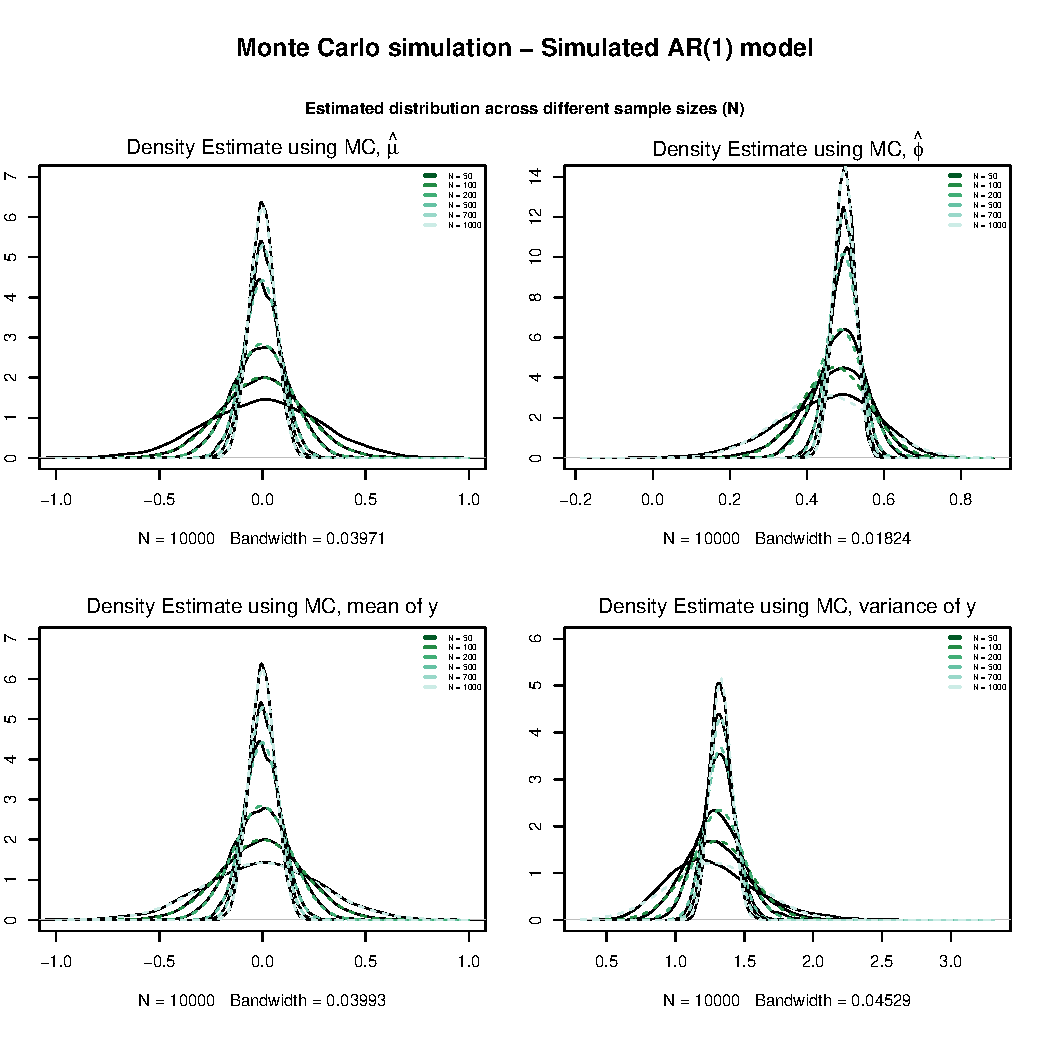
\includegraphics[width=\textwidth]{plots/MC_AR1_densities_diff_smpl}
\caption{MC simulation for an $AR(1)$ model: changing the sample size}
\label{fig:MC_AR1_densities_diff_smpl}
\centering
\end{figure}

\begin{figure}[hbt!]
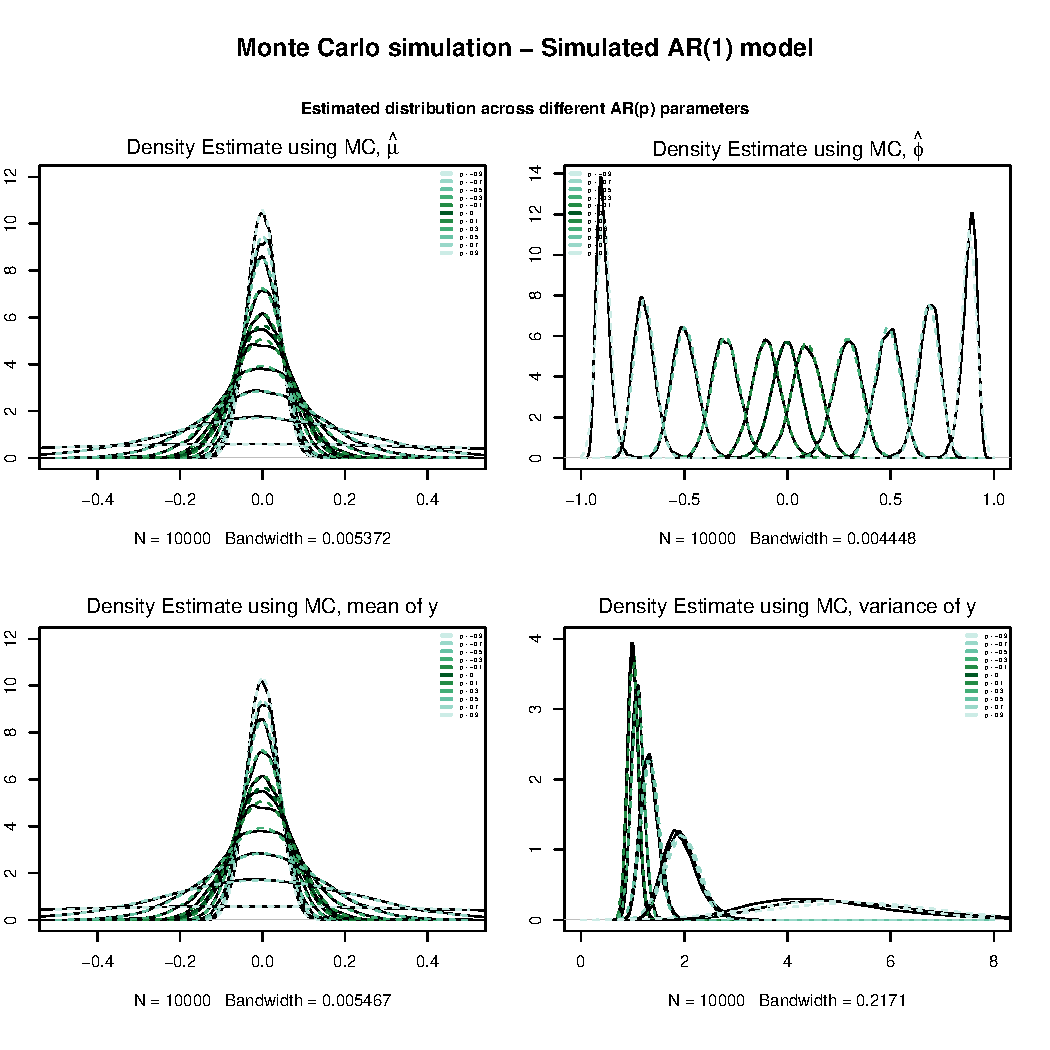
\includegraphics[width=\textwidth]{plots/MC_AR1_densities_diff_ARq}
\caption{MC simulation for an $AR(1)$ model: changing the autoregressive parameter}
\label{fig:MC_AR1_densities_diff_ARq}
\centering
\end{figure}

\begin{figure}[hbt!]
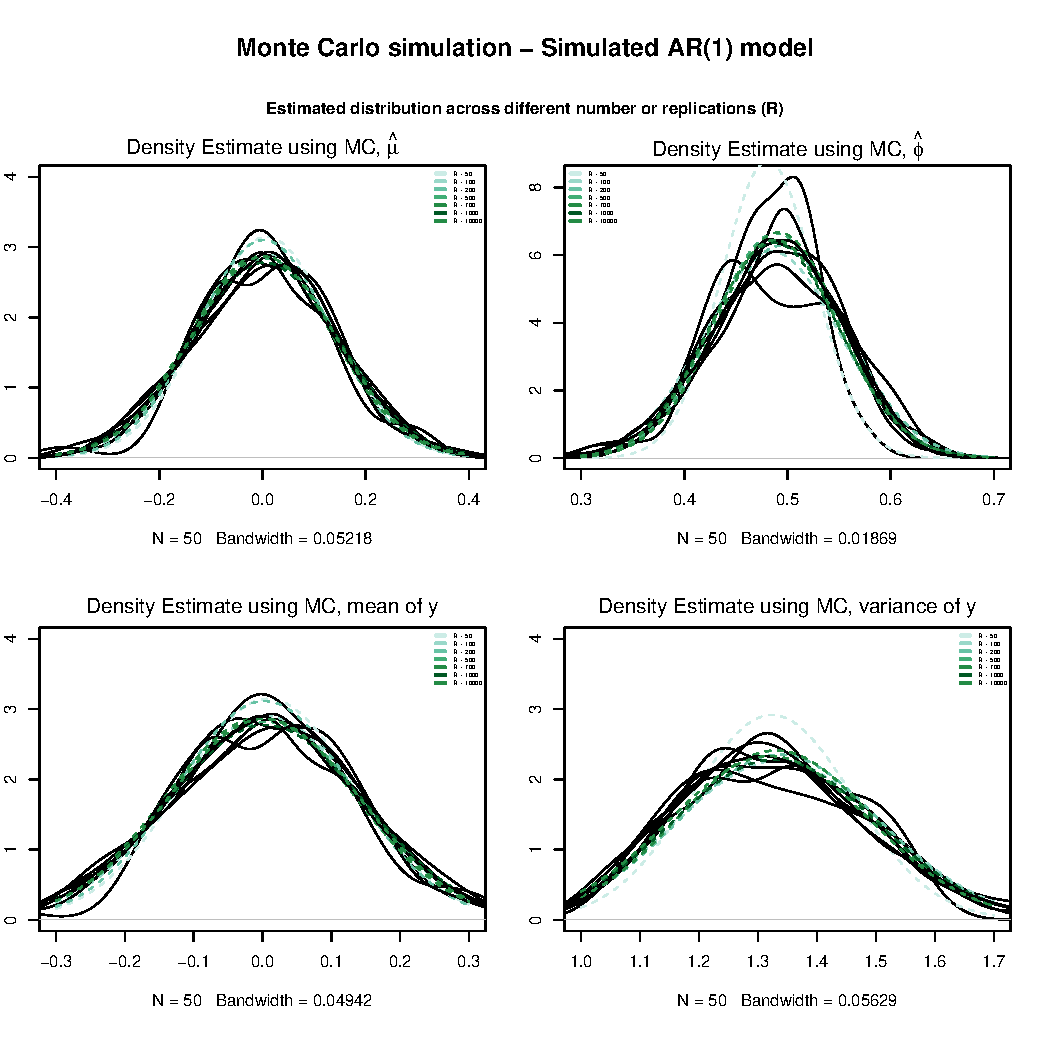
\includegraphics[width=\textwidth]{plots/MC_AR1_densities_diff_norepl}
\caption{MC simulation for an $AR(1)$ model: changing the number of replications}
\label{fig:MC_AR1_densities_diff_norepl}
\centering
\end{figure}


\clearpage
\subsubsection{$MA(1)$ models}
\begin{figure}[hbt!]
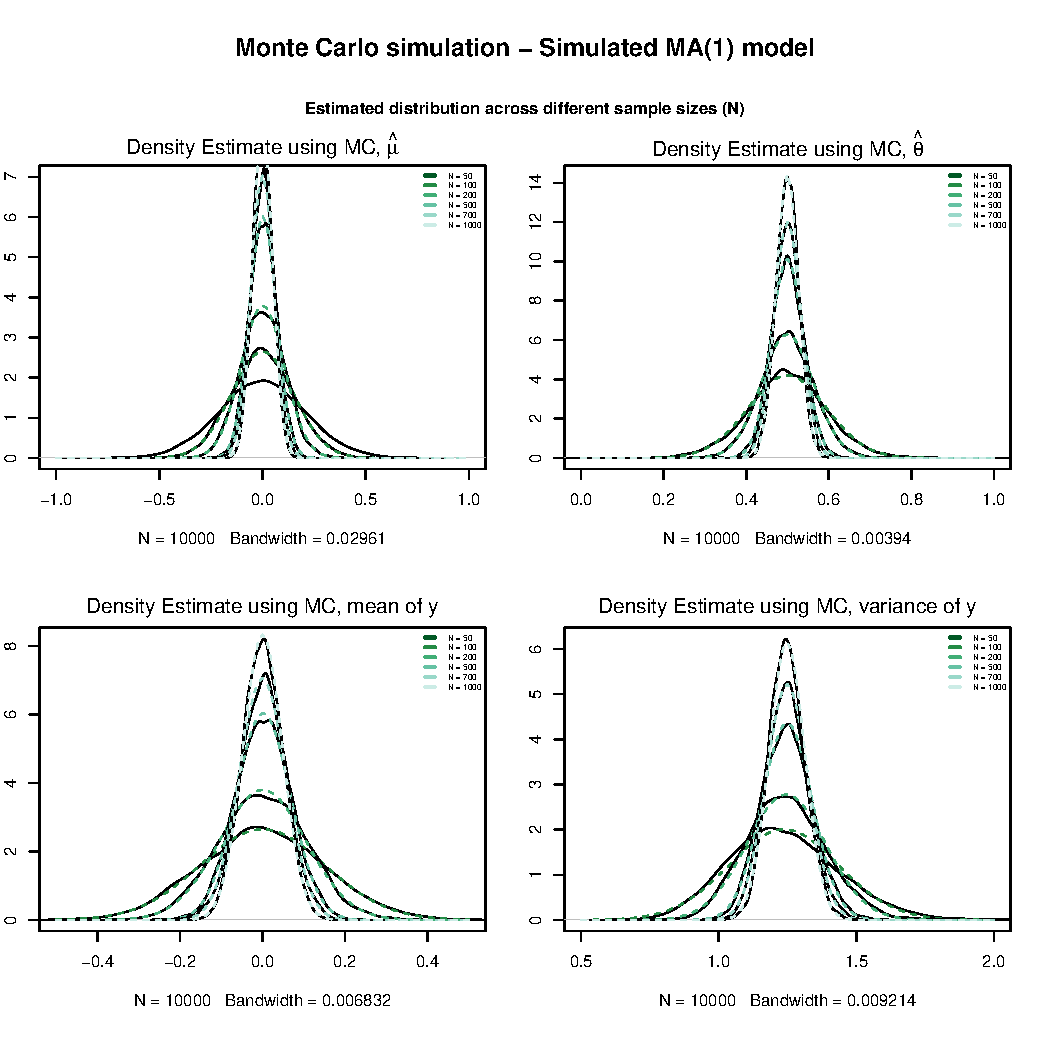
\includegraphics[width=\textwidth]{plots/MC_MA1_densities_diff_smpl}
\caption{MC simulation for an $MA(1)$ model: changing the sample size}
\label{fig:MC_MA1_densities_diff_smpl}
\centering
\end{figure}

\begin{figure}[hbt!]
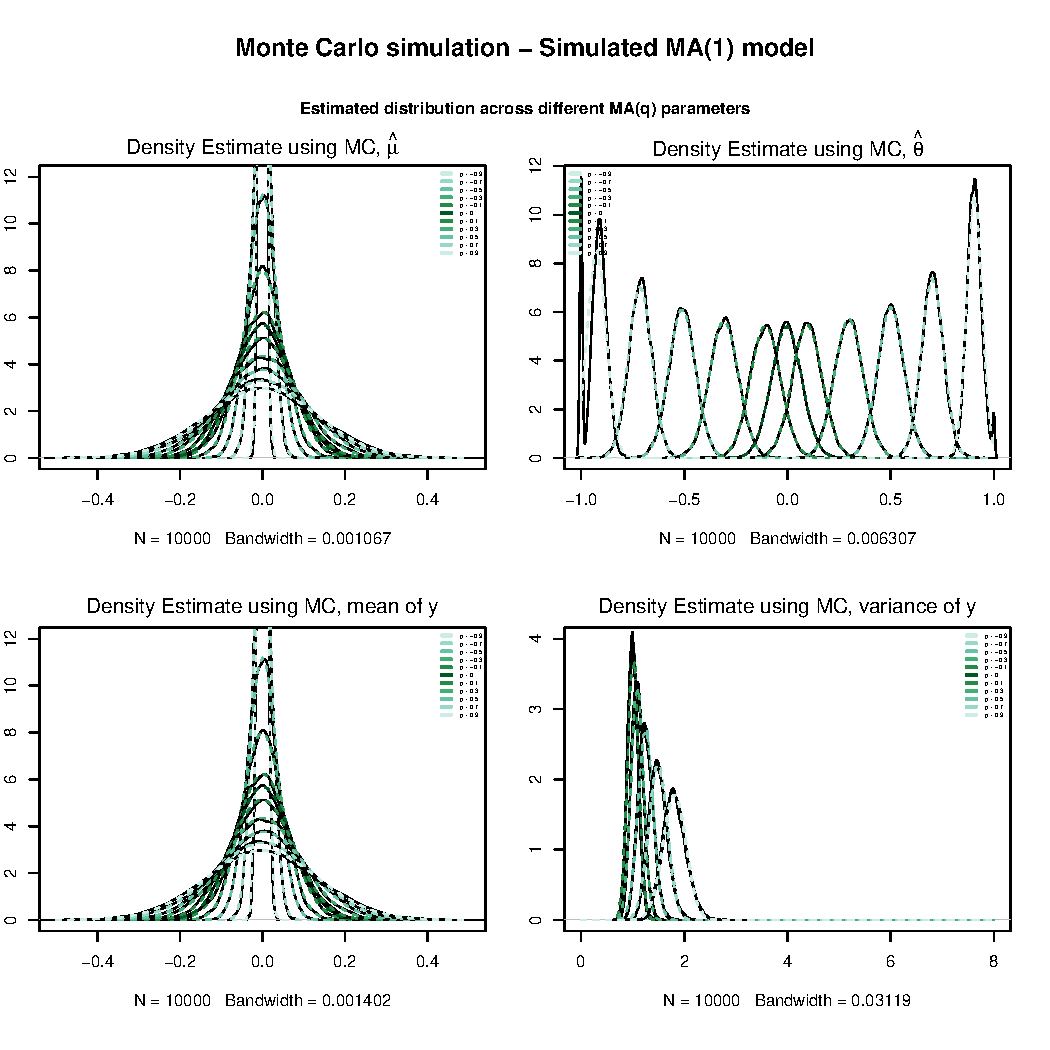
\includegraphics[width=\textwidth]{plots/MC_MA1_densities_diff_ARq}
\caption{MC simulation for an $MA(1)$ model: changing the autoregressive parameter}
\label{fig:MC_MA1_densities_diff_ARq}
\centering
\end{figure}

\begin{figure}[hbt!]
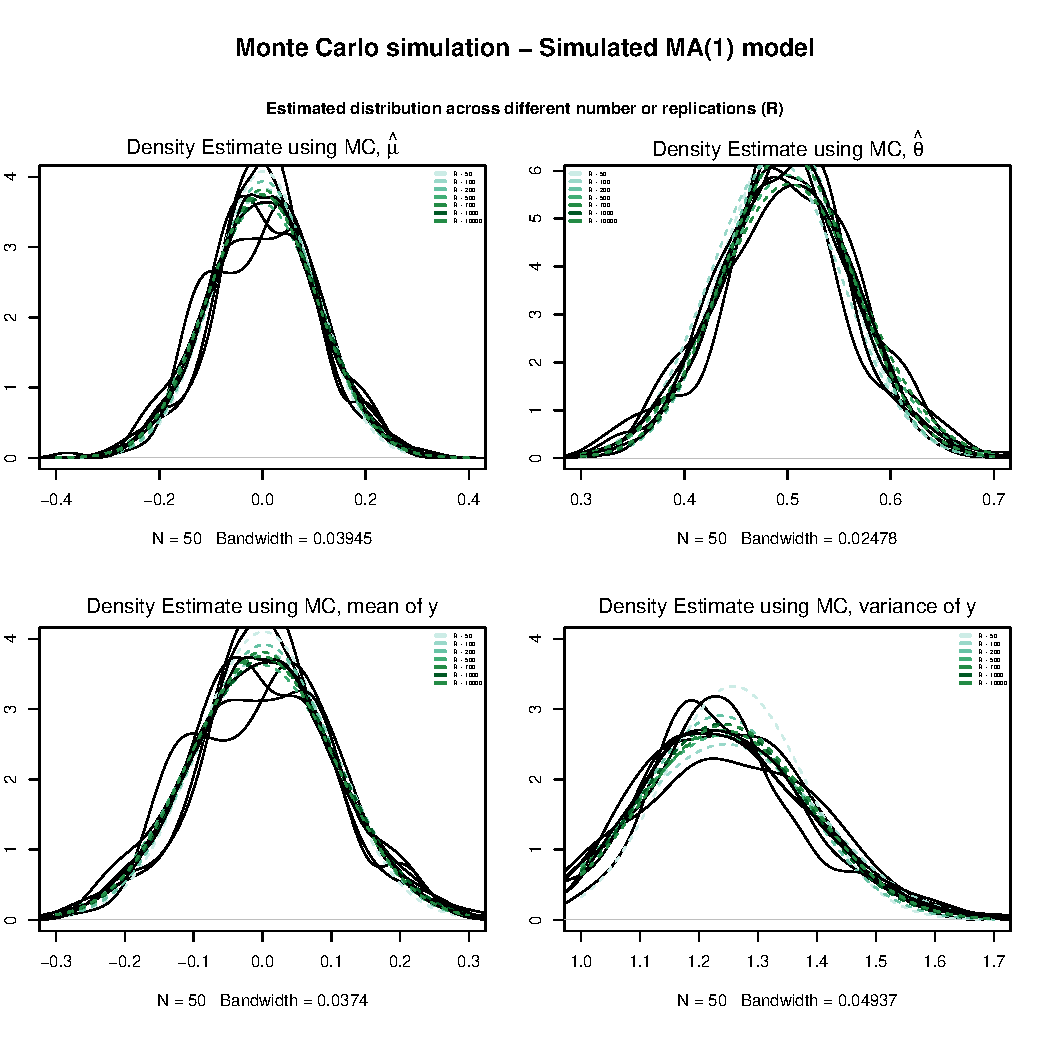
\includegraphics[width=\textwidth]{plots/MC_MA1_densities_diff_norepl}
\caption{MC simulation for an $MA(1)$ model: changing the number of replications}
\label{fig:MC_MA1_densities_diff_norepl}
\centering
\end{figure}



\clearpage
%%%%%%%%%%%%%%%%%%%%%%

\begin{figure}[hbt!]
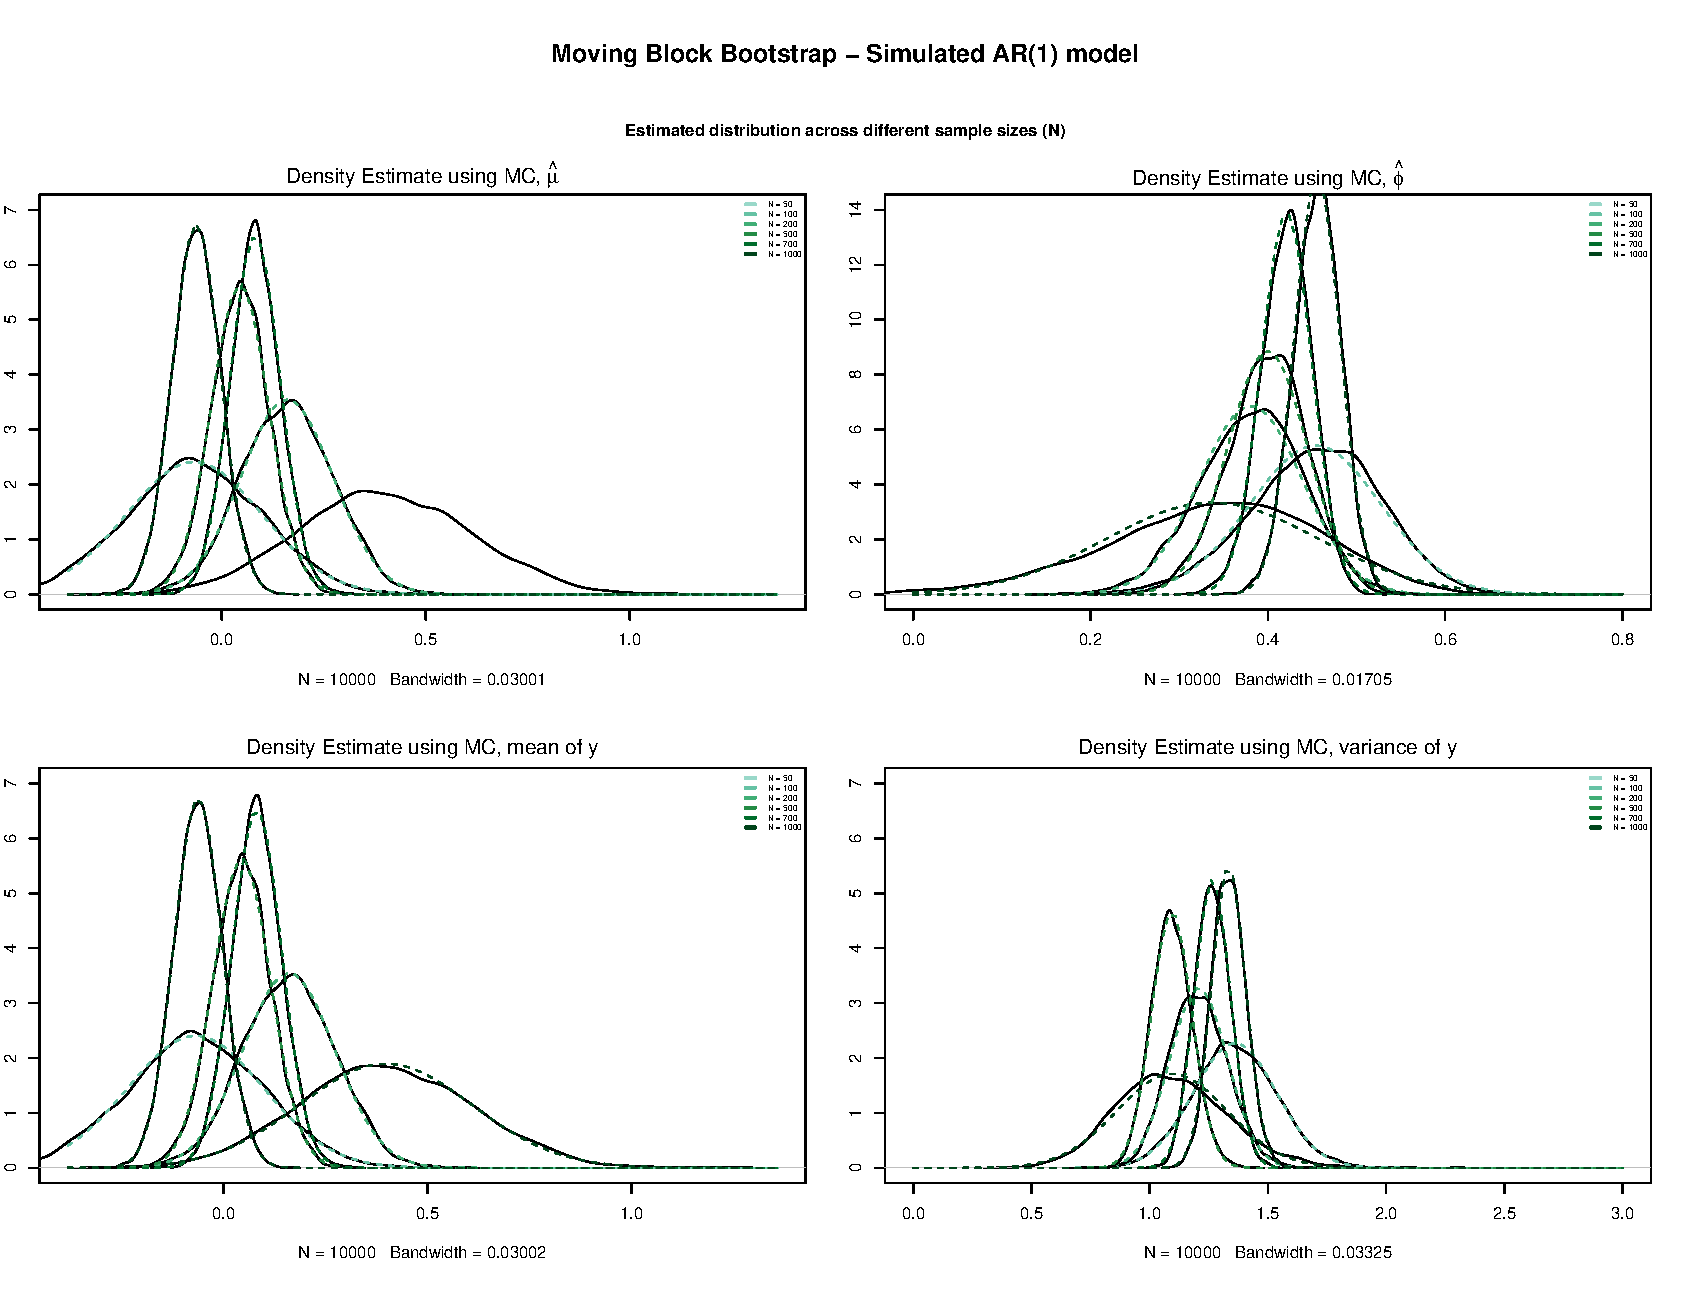
\includegraphics[width=\textwidth]{plots/MBB_AR1_densities_diff_smpl}
\caption{MBB for an $AR(1)$ model: changing the sample size}
\label{fig:MBB_AR1_densities_diff_smpl}
\centering
\end{figure}

\begin{figure}[hbt!]
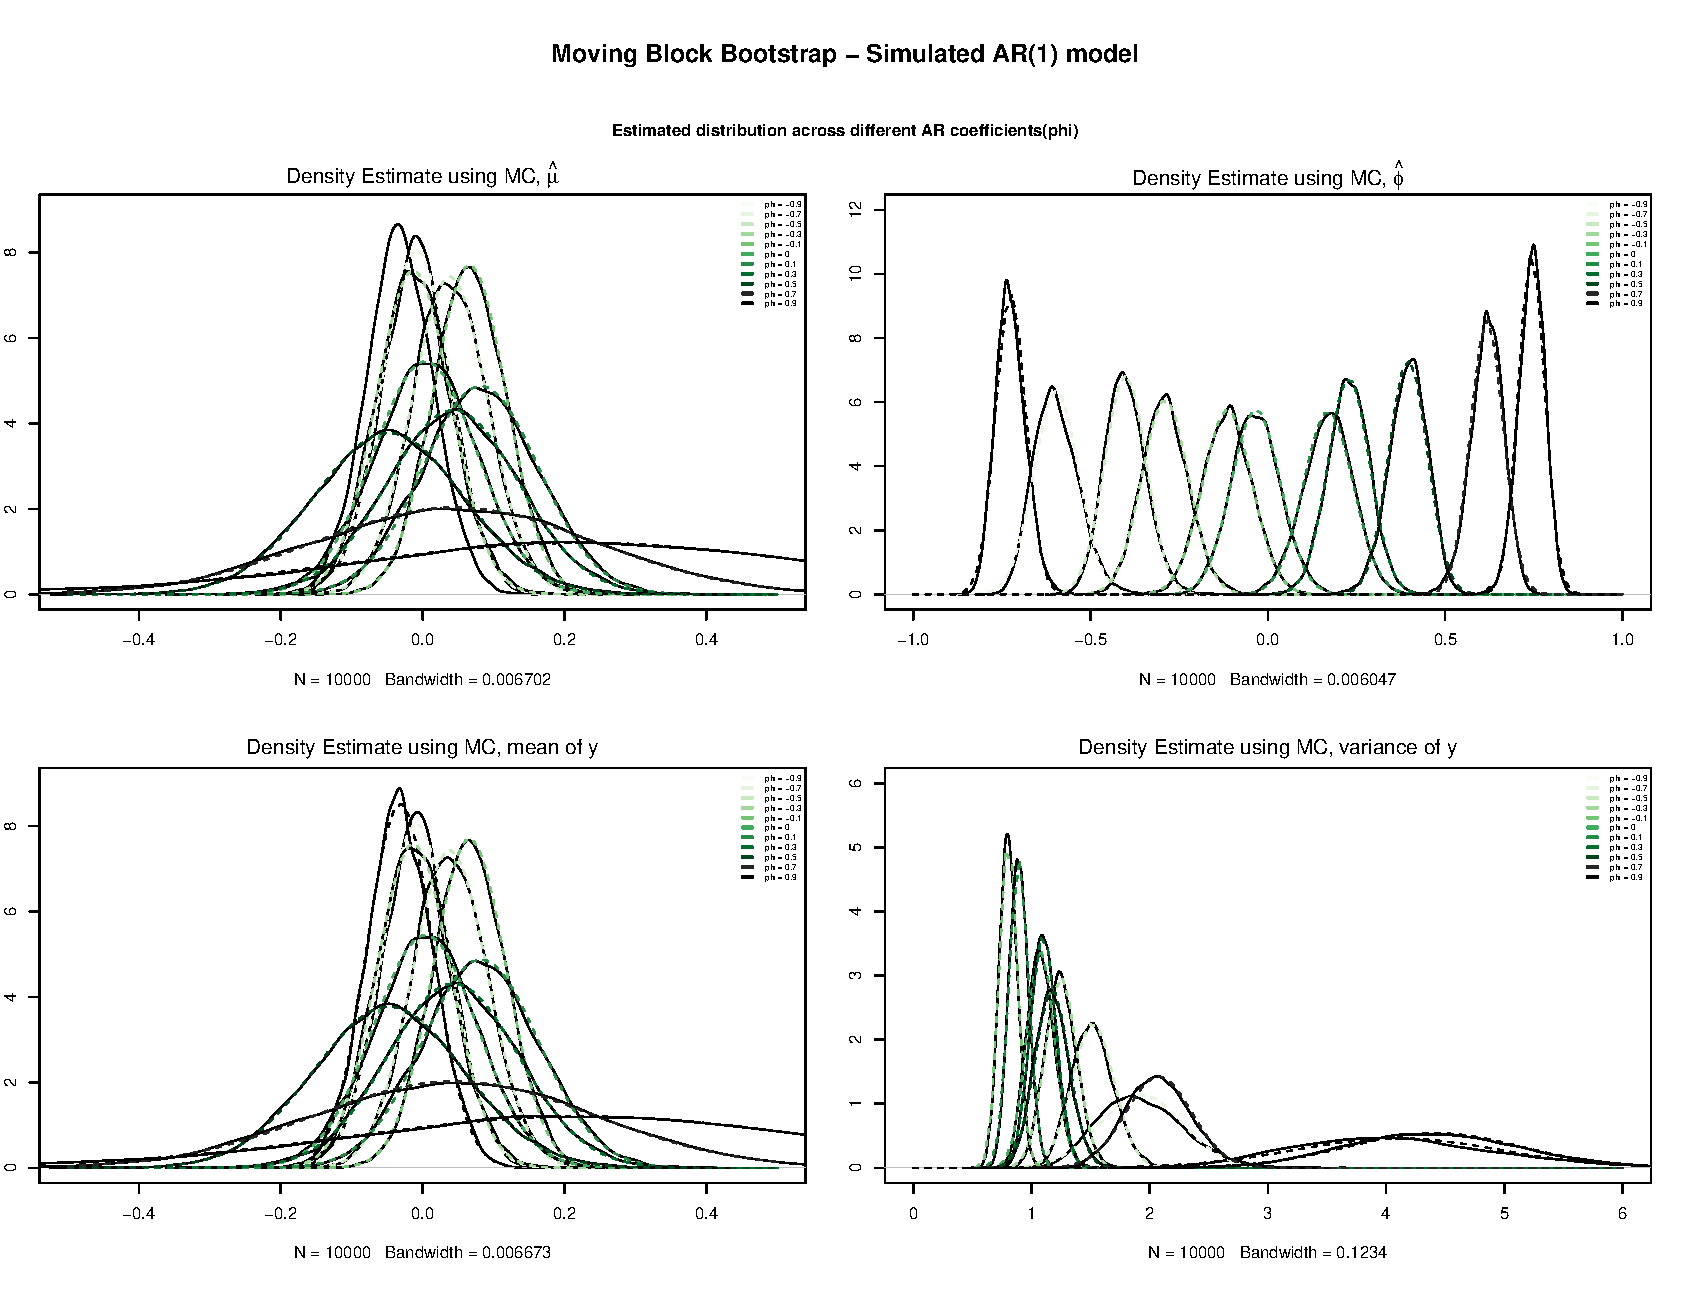
\includegraphics[width=\textwidth]{plots/MBB_AR1_densities_diff_ARq}
\caption{MBB for an $AR(1)$ model: changing the autoregressive parameter}
\label{fig:MBB_AR1_densities_diff_ARq}
\centering
\end{figure}

\begin{figure}[hbt!]
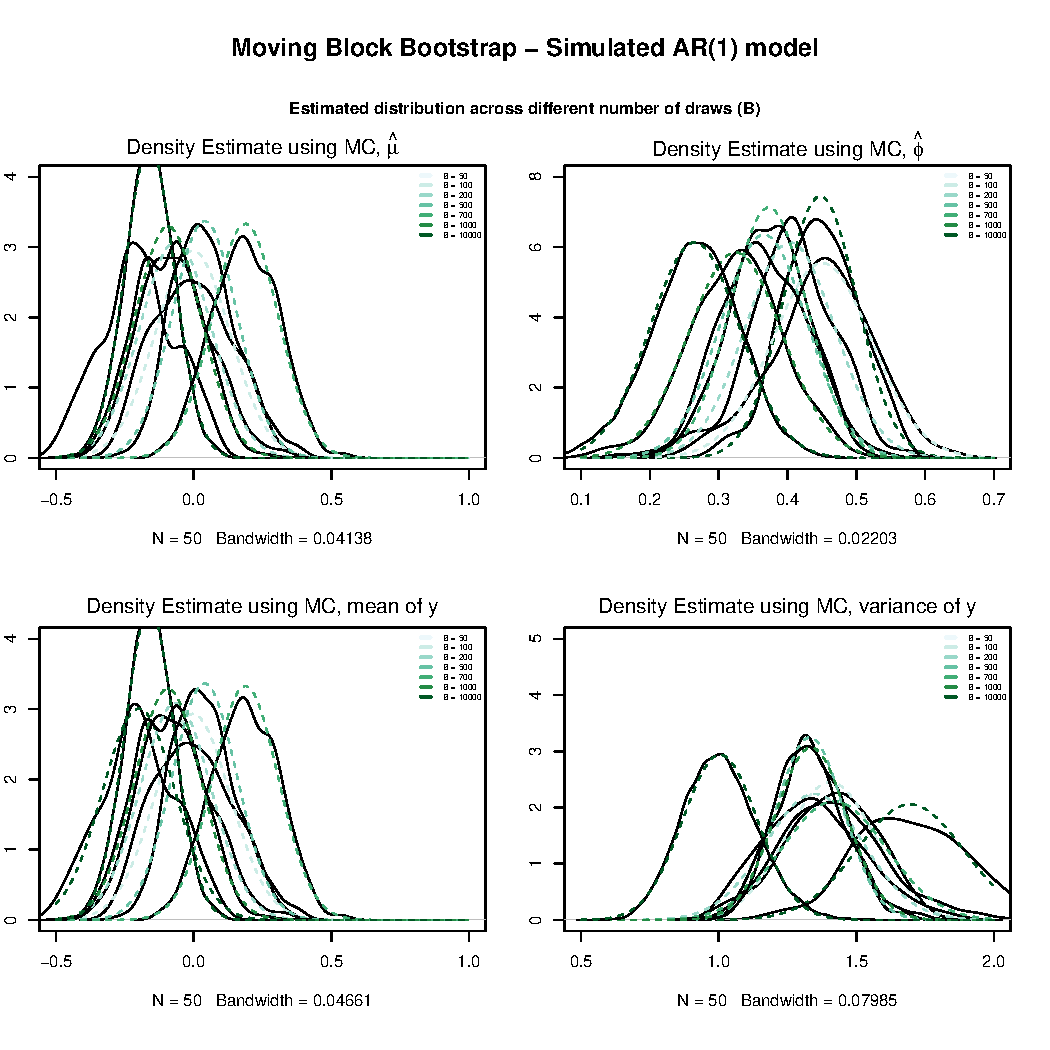
\includegraphics[width=\textwidth]{plots/MBB_AR1_densities_diff_drawsB}
\caption{MBB for an $AR(1)$ model: changing the number of draws}
\label{fig:MBB_AR1_densities_diff_drawsB}
\centering
\end{figure}

\begin{figure}[hbt!]
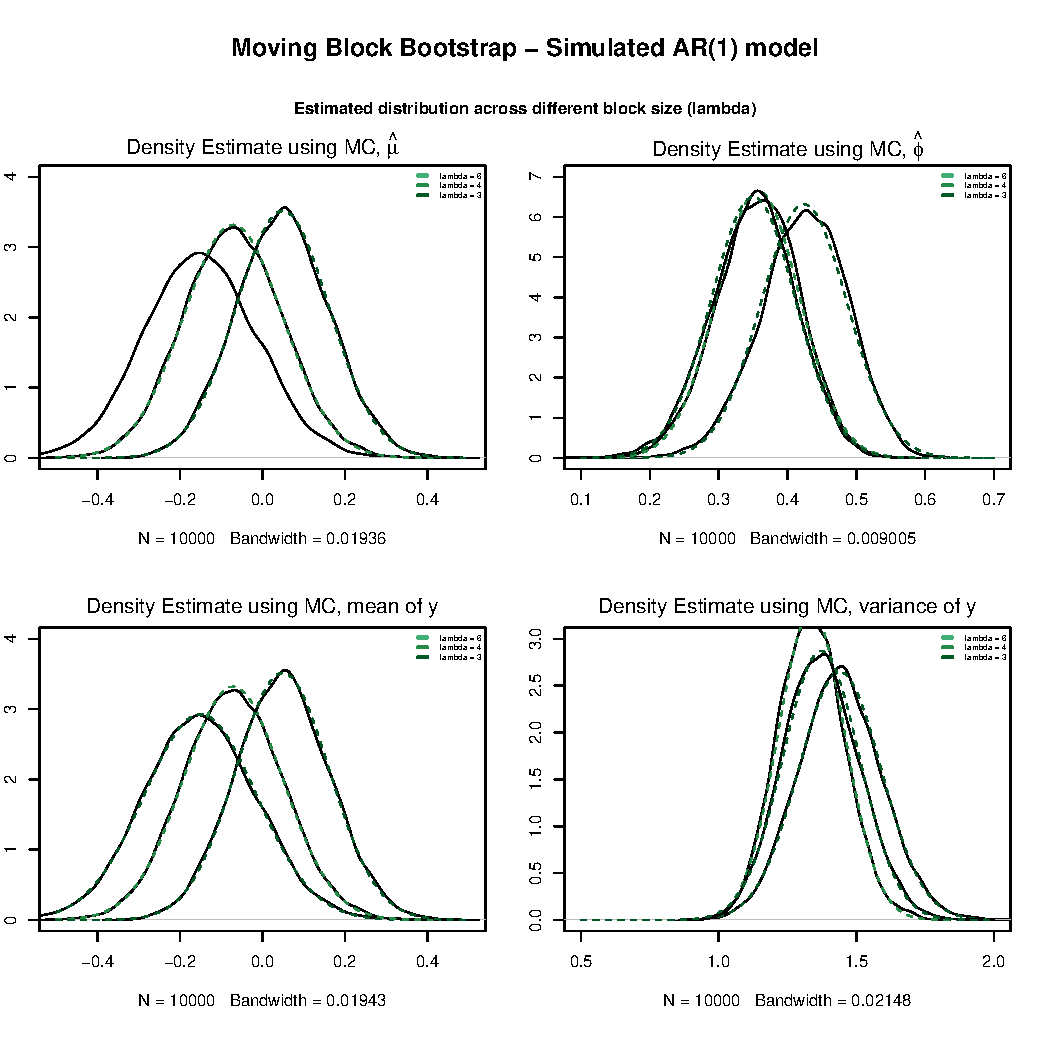
\includegraphics[width=\textwidth]{plots/MBB_AR1_densities_diff_blocklength}
\caption{MBB for an $AR(1)$ model: changing the block length}
\label{fig:MBB_AR1_densities_diff_blocklength}
\centering
\end{figure}


\clearpage
%%%%%%%%%%%%%%%%%%%%%%
\begin{figure}[hbt!]
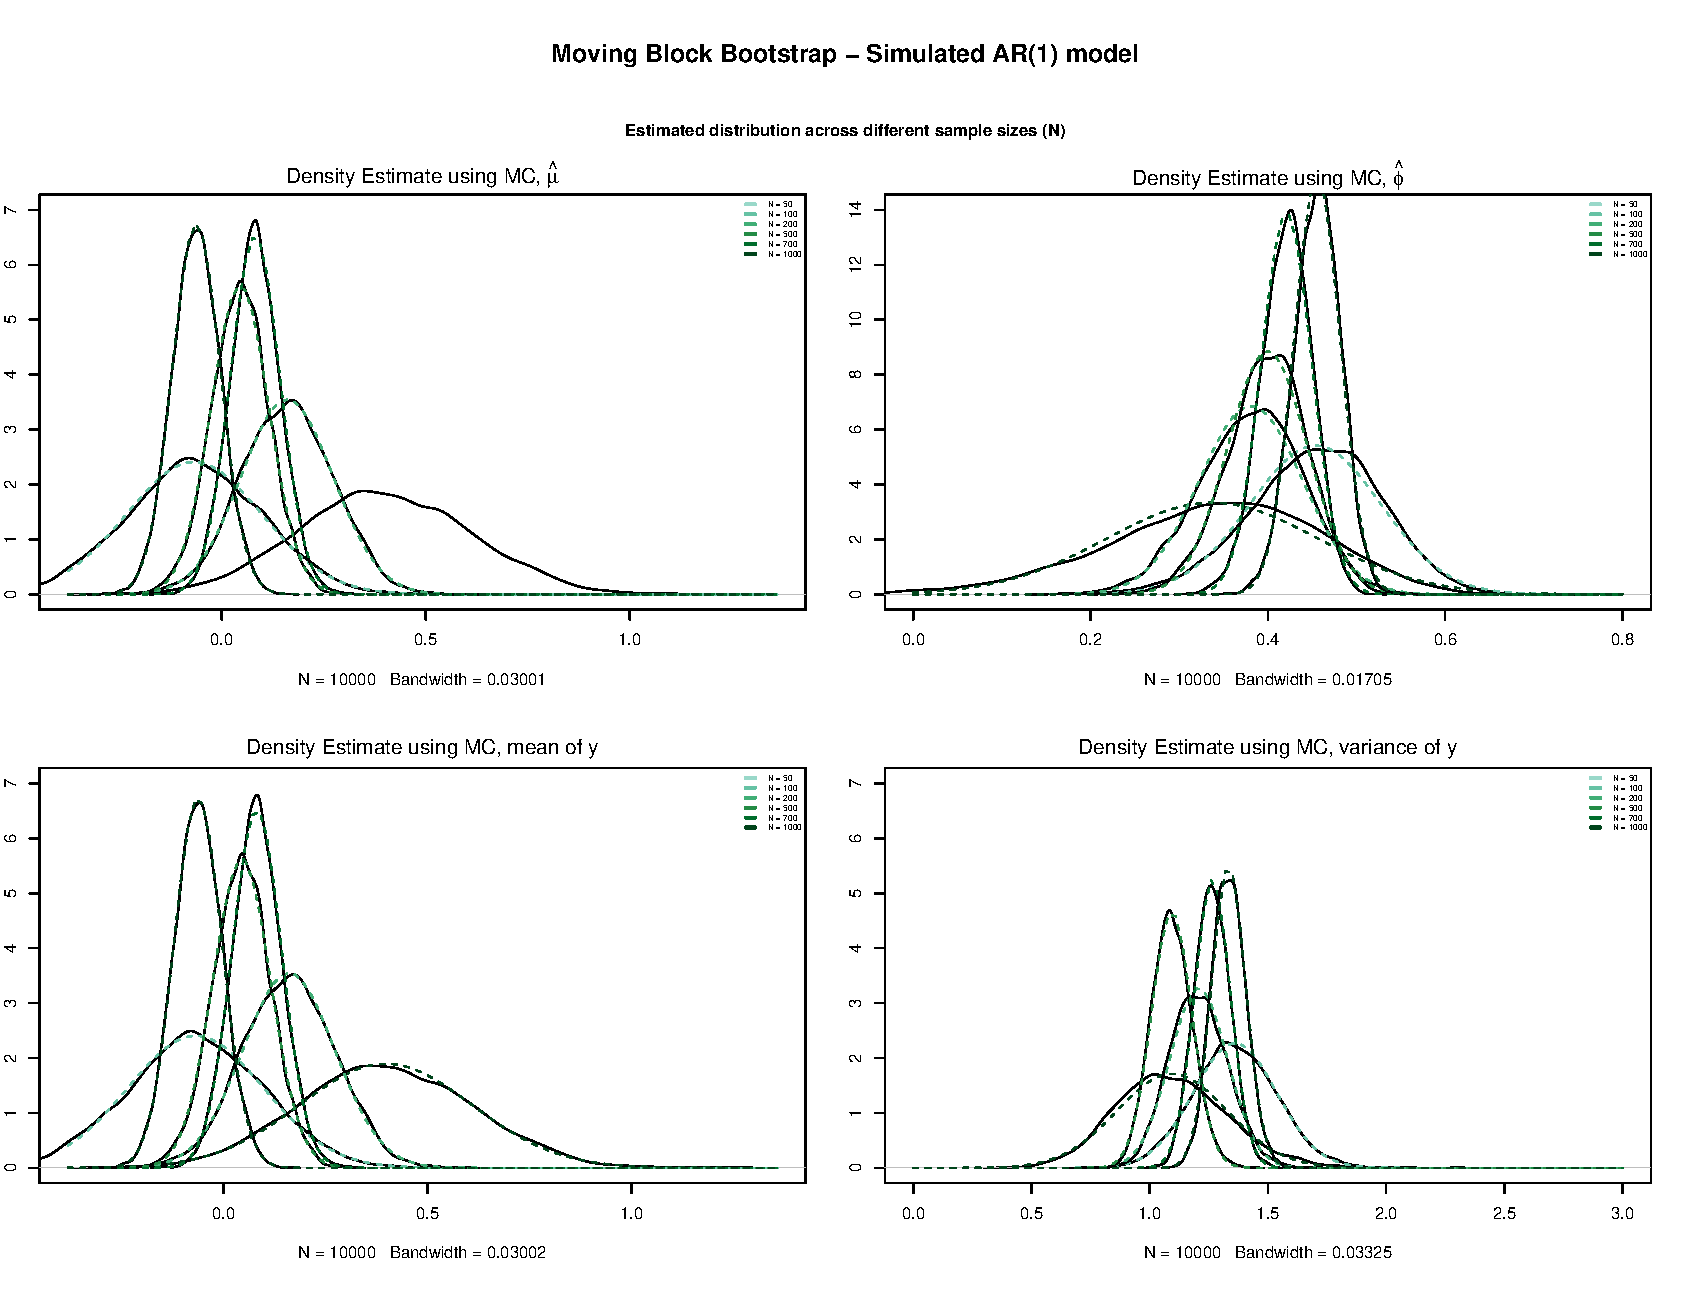
\includegraphics[width=\textwidth]{plots/MBB_AR1_densities_diff_smpl}
\caption{MBB for an $MA(1)$ model: changing the sample size}
\label{fig:MBB_MA1_densities_diff_smpl}
centering
\end{figure}

\begin{figure}[hbt!]
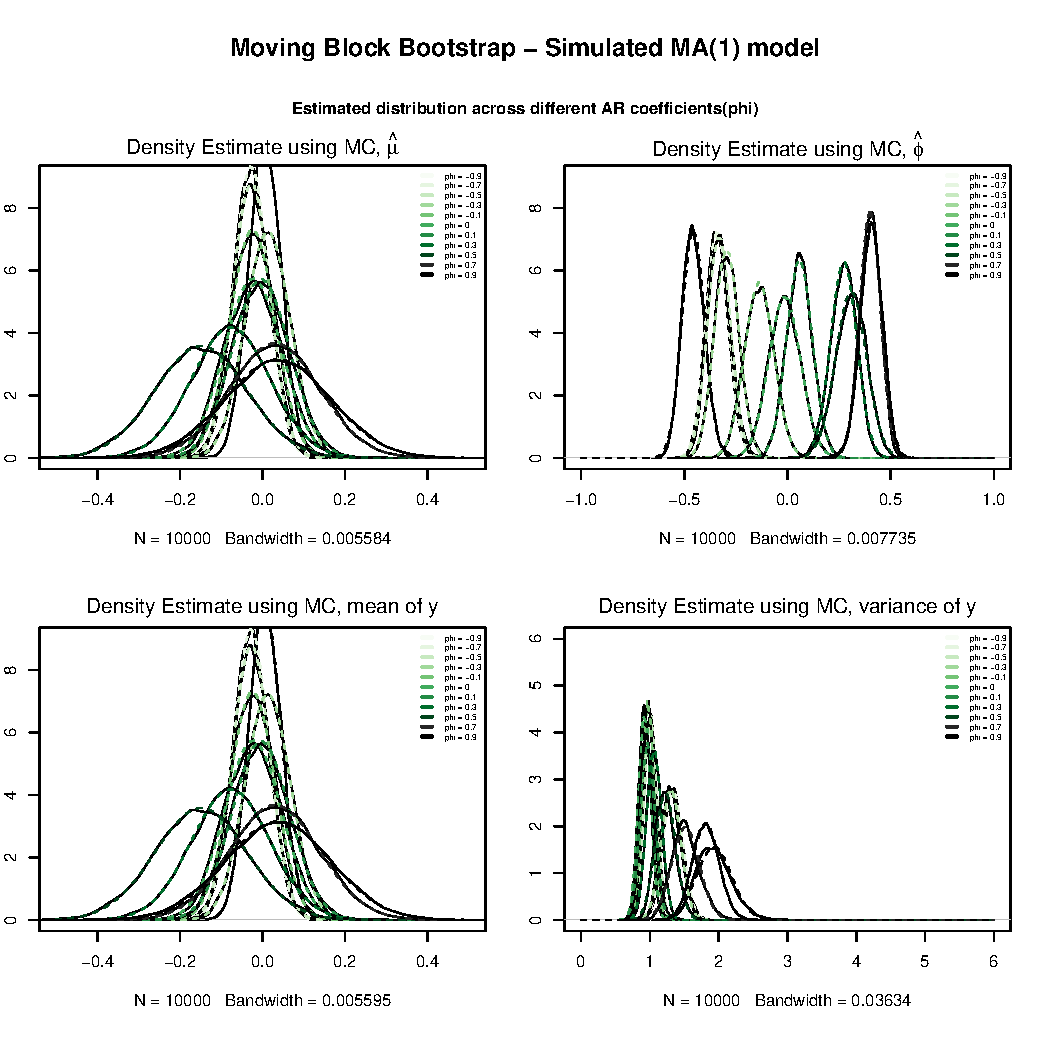
\includegraphics[width=\textwidth]{plots/MBB_MA1_densities_diff_ARq}
\caption{MBB for an $MA(1)$ model: changing the autoregressive parameter}
\label{fig:MBB_MA1_densities_diff_ARq}
\centering
\end{figure}

\begin{figure}[hbt!]
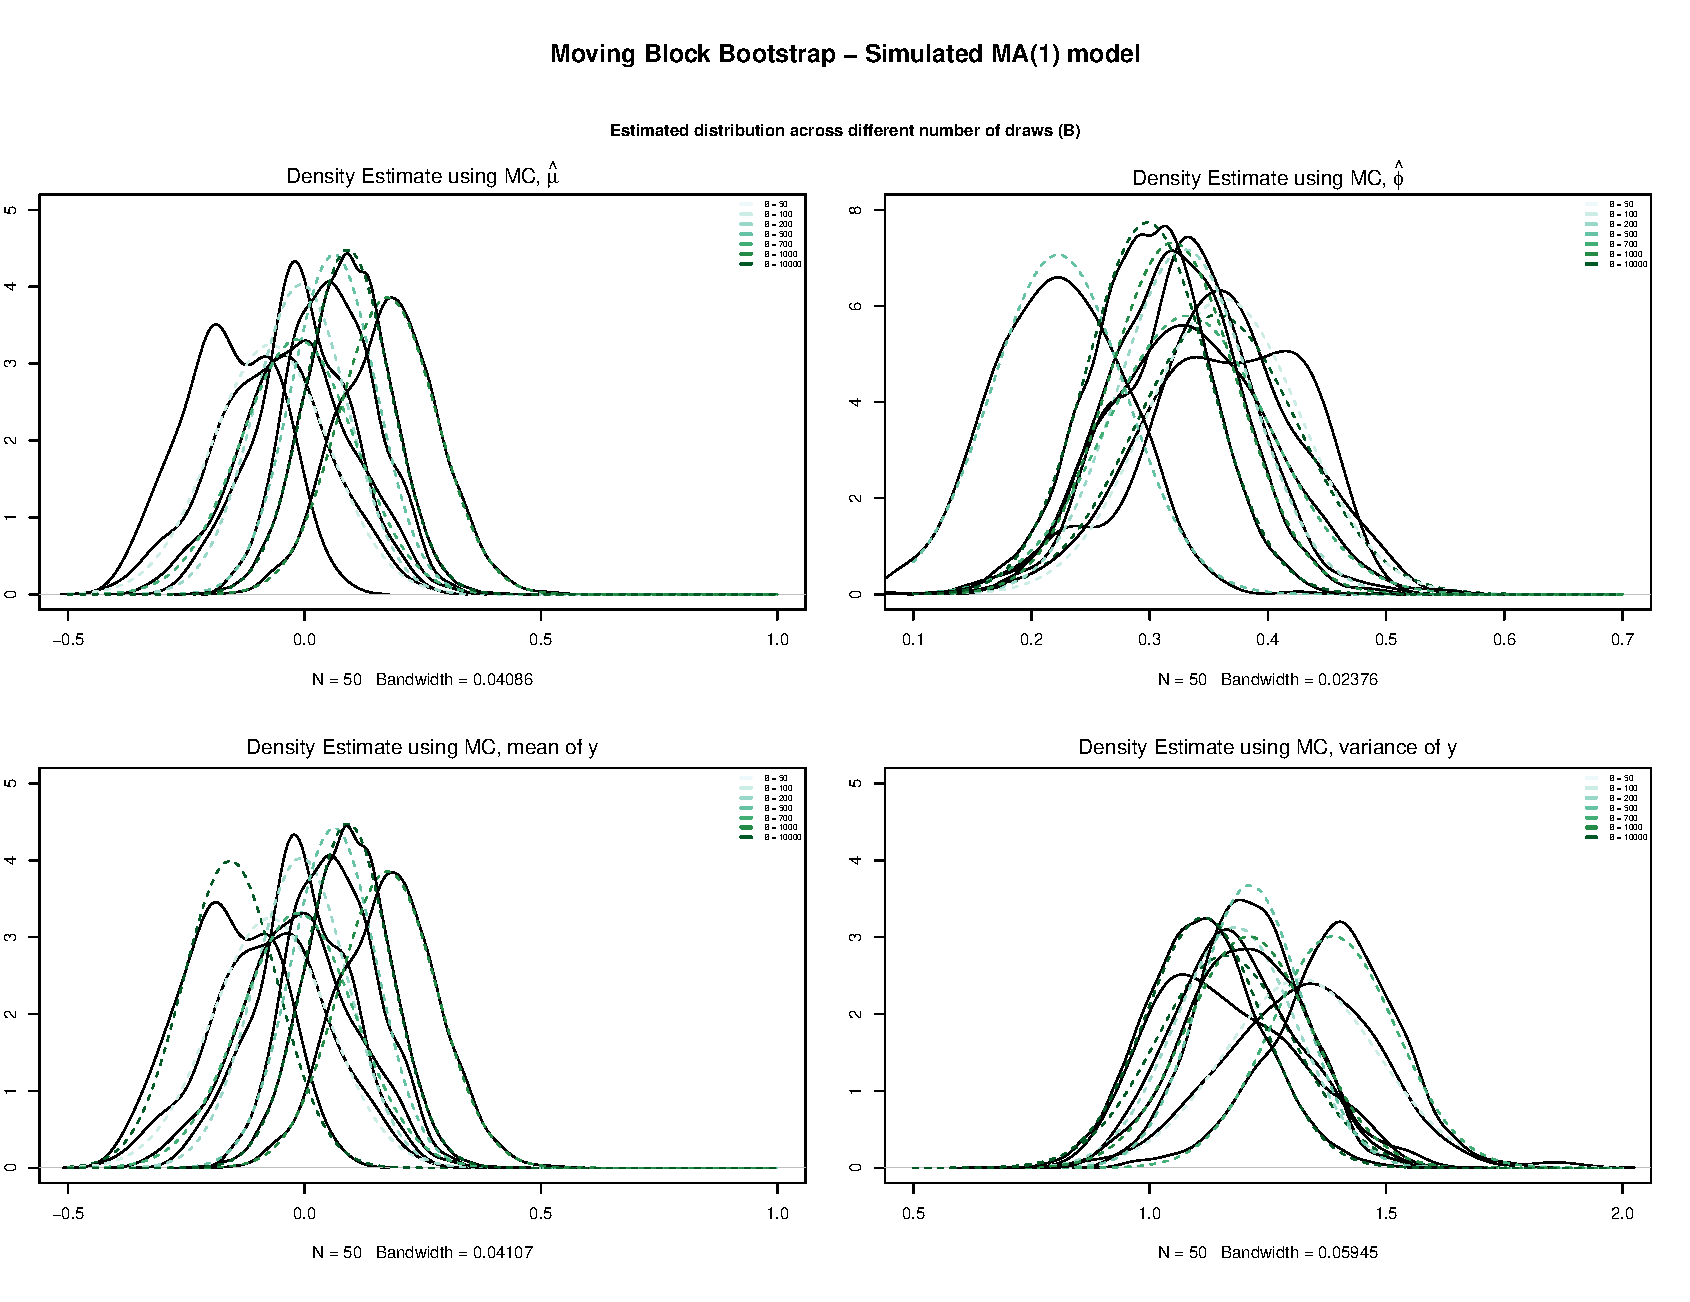
\includegraphics[width=\textwidth]{plots/MBB_MA1_densities_diff_drawsB}
\caption{MBB for an $MA(1)$ model: changing the number of draws}
\label{fig:MBB_MA1_densities_diff_drawsB}
\centering
\end{figure}

\begin{figure}[hbt!]
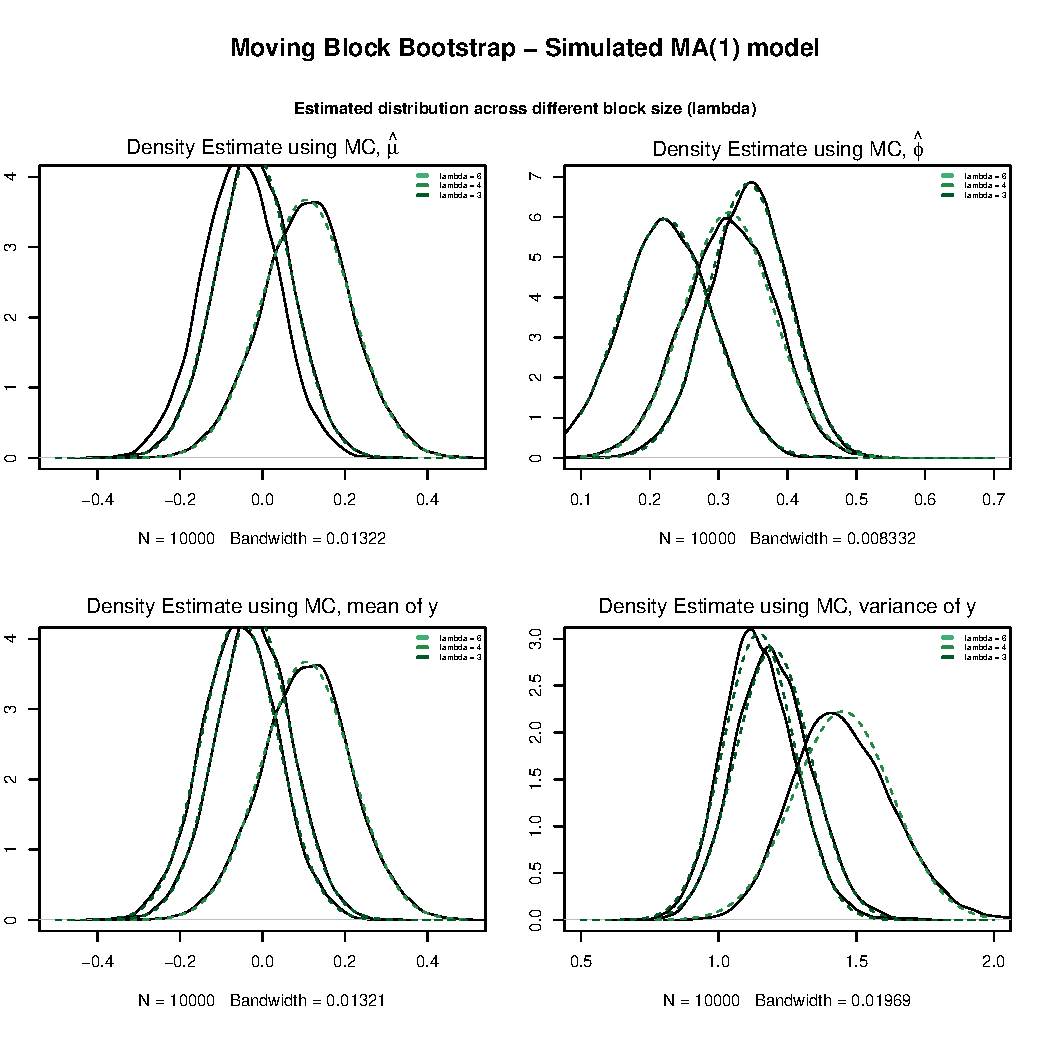
\includegraphics[width=\textwidth]{plots/MBB_MA1_densities_diff_blocklength}
\caption{MBB for an $MA(1)$ model: changing the block length}
\label{fig:MBB_MA1_densities_diff_blocklength}
\centering
\end{figure}


\clearpage
%%%%%%%%%%%%%%%%%%%%%%
\begin{subfigures}
\begin{figure}[hbt!]
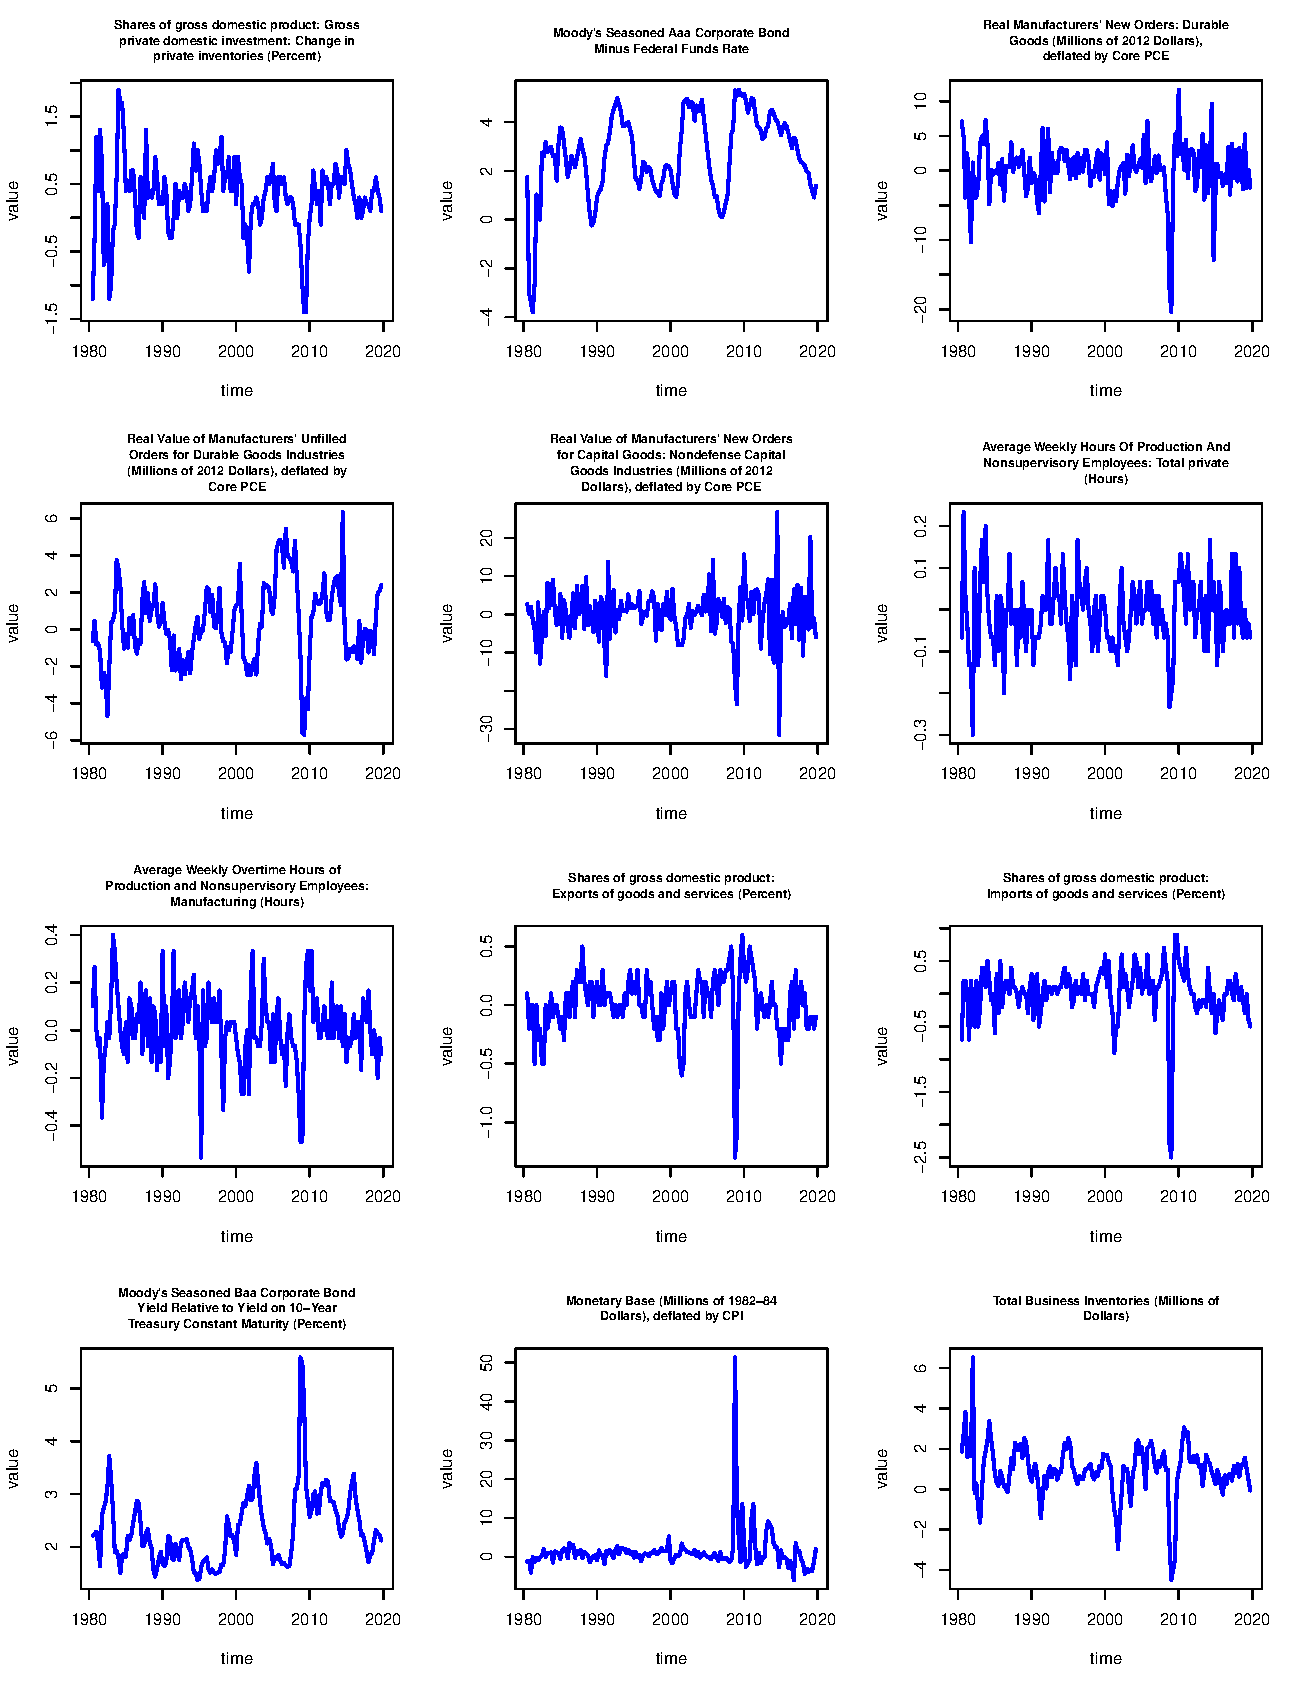
\includegraphics[page = 1, width=\textwidth]{plots/transformed_series}
\caption{\label{first}FRED-QD transformed series}
\label{fig:transformed_series_1}
\centering
\end{figure}

\begin{figure}[hbt!]
\includegraphics[page = 2, width=\textwidth]{plots/transformed_series}
\caption{\label{second}FRED-QD transformed series}
\label{fig:transformed_series_2}
\centering
\end{figure}

\begin{figure}[hbt!]
\includegraphics[page = 3, width=\textwidth]{plots/transformed_series}
\caption{\label{third}FRED-QD transformed series}
\label{fig:transformed_series_3}
\centering
\end{figure}

\begin{figure}[hbt!]
\includegraphics[page = 4, width=\textwidth]{plots/transformed_series}
\caption{\label{fourth}FRED-QD transformed series}
\label{fig:transformed_series_4}
\centering
\end{figure}

\begin{figure}[hbt!]
\includegraphics[page = 5, width=\textwidth]{plots/transformed_series}
\caption{\label{fifth}FRED-QD transformed series}
\label{fig:transformed_series_5}
\centering
\end{figure}

\begin{figure}[hbt!]
\includegraphics[page = 6, width=\textwidth]{plots/transformed_series}
\caption{\label{sixth}FRED-QD transformed series}
\label{fig:transformed_series_6}
\centering
\end{figure}

\begin{figure}[hbt!]
\includegraphics[page = 7, width=\textwidth]{plots/transformed_series}
\label{fig:transformed_series_7}
\caption{\label{seventh}FRED-QD transformed series}
\centering
\end{figure}

\begin{figure}[hbt!]
\includegraphics[page = 8, width=\textwidth]{plots/transformed_series}
\caption{\label{eighth}FRED-QD transformed series}
\label{fig:transformed_series_8}
\centering
\end{figure}

\begin{figure}[hbt!]
\includegraphics[page = 9, width=\textwidth]{plots/transformed_series}
\label{fig:transformed_series_9}
\caption{\label{ninth}FRED-QD transformed series}
\centering
\end{figure}

\begin{figure}[hbt!]
\includegraphics[page = 10, width=\textwidth]{plots/transformed_series}
\caption{\label{tenth}FRED-QD transformed series}
\label{fig:transformed_series_10}
\centering
\end{figure}

\begin{figure}[hbt!]
\includegraphics[page = 11, width=\textwidth]{plots/transformed_series}
\caption{\label{eleventh}FRED-QD transformed series}
\label{fig:transformed_series_11}
\centering
\end{figure}

\begin{figure}[hbt!]
\includegraphics[page = 12, width=\textwidth]{plots/transformed_series}
\caption{\label{twelfth}FRED-QD transformed series}
\label{fig:transformed_series_12}
\centering
\end{figure}
   
\begin{figure}[hbt!]
\includegraphics[page = 13, width=\textwidth]{plots/transformed_series}
\label{fig:transformed_series_13}
\caption{\label{thirteenth}FRED-QD transformed series}
\centering
\end{figure}

\begin{figure}[hbt!]
\includegraphics[page = 14, width=\textwidth]{plots/transformed_series}
\label{fig:transformed_series_14}
\caption{\label{fourteenth}FRED-QD transformed series}
\centering
\end{figure}

\begin{figure}[hbt!]
\includegraphics[page = 15, width=\textwidth]{plots/transformed_series}
\label{fig:transformed_series_15}
\caption{\label{fifteenth}FRED-QD transformed series}
\centering
\end{figure}

\begin{figure}[hbt!]
\includegraphics[page = 16, width=\textwidth]{plots/transformed_series}
\label{fig:transformed_series_16}
\caption{\label{sixteenth}FRED-QD transformed series}
\centering
\end{figure}

\begin{figure}[hbt!]
\includegraphics[page = 17, width=\textwidth]{plots/transformed_series}
\label{fig:transformed_series_17}
\caption{\label{seventeenth}FRED-QD transformed series}
\centering
\end{figure}


\end{subfigures}


\clearpage
%%%%%%%%%%%%%%%%%%%%%%
\begin{subfigures}
\begin{figure}[hbt!]
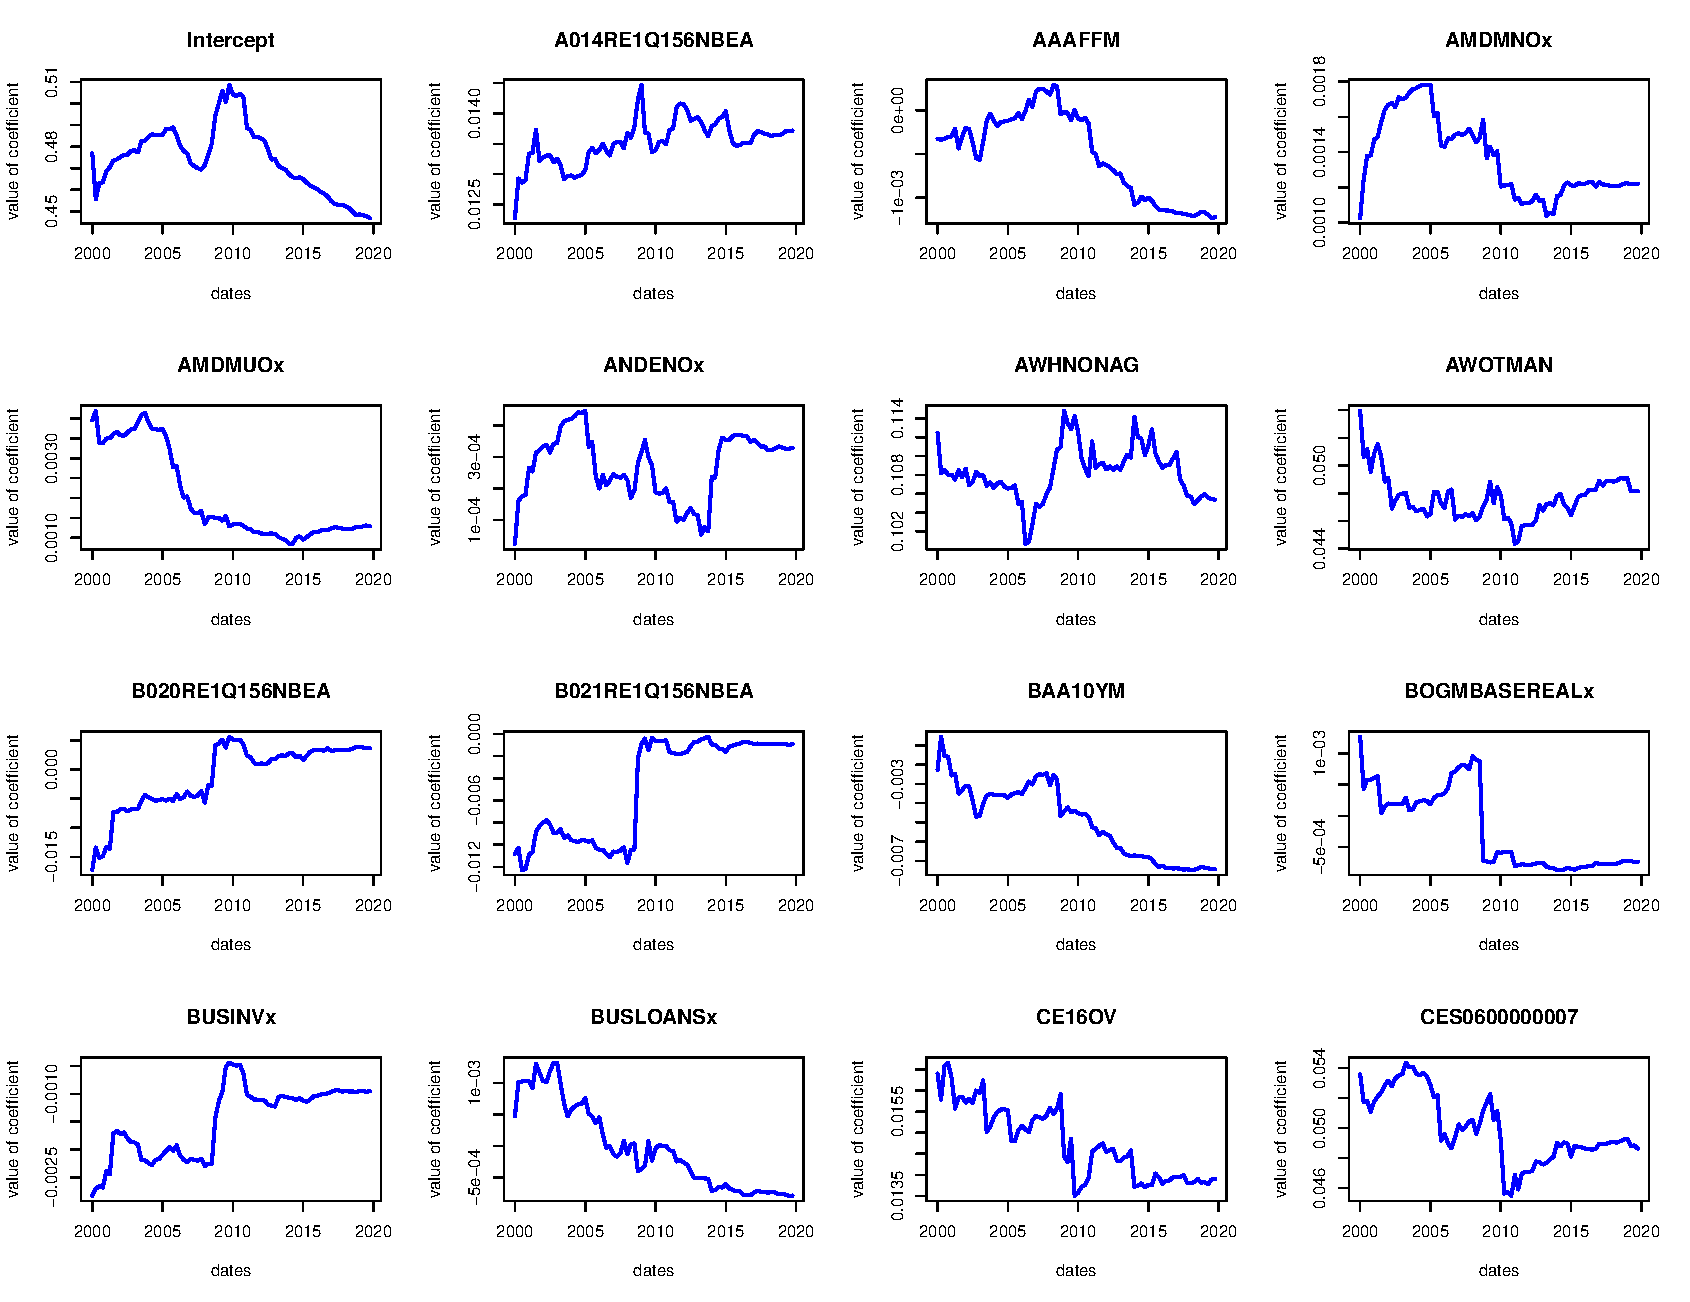
\includegraphics[page = 1, width=\textwidth]{plots/ridge_betas}
\caption{\label{first}Ridge regression: The evolution of the estimated $\beta$ coefficients over time}
\label{fig:ridge_betas}
\centering
\end{figure}

\begin{figure}[hbt!]
\includegraphics[page = 2, width=\textwidth]{plots/ridge_betas}
\caption{\label{second}Ridge regression: The evolution of the estimated $\beta$ coefficients over time}
\label{fig:ridge_betas}
\centering
\end{figure}

\begin{figure}[hbt!]
\includegraphics[page = 3, width=\textwidth]{plots/ridge_betas}
\caption{\label{third}Ridge regression: The evolution of the estimated $\beta$ coefficients over time}
\label{fig:ridge_betas}
\centering
\end{figure}

\begin{figure}[hbt!]
\includegraphics[page = 4, width=\textwidth]{plots/ridge_betas}
\caption{\label{fourth}Ridge regression: The evolution of the estimated $\beta$ coefficients over time}
\label{fig:ridge_betas}
\centering
\end{figure}

\begin{figure}[hbt!]
\includegraphics[page = 5, width=\textwidth]{plots/ridge_betas}
\caption{\label{fifth}Ridge regression: The evolution of the estimated $\beta$ coefficients over time}
\label{fig:ridge_betas}
\centering
\end{figure}

\begin{figure}[hbt!]
\includegraphics[page = 6, width=\textwidth]{plots/ridge_betas}
\caption{\label{sixth}Ridge regression: The evolution of the estimated $\beta$ coefficients over time}
\label{fig:ridge_betas}
\centering
\end{figure}

\begin{figure}[hbt!]
\includegraphics[page = 7, width=\textwidth]{plots/ridge_betas}
\label{fig:ridge_betas}
\caption{\label{seventh}Ridge regression: The evolution of the estimated $\beta$ coefficients over time}
\centering
\end{figure}

\begin{figure}[hbt!]
\includegraphics[page = 8, width=\textwidth]{plots/ridge_betas}
\caption{\label{eighth}Ridge regression: The evolution of the estimated $\beta$ coefficients over time}
\label{fig:ridge_betas}
\centering
\end{figure}

\begin{figure}[hbt!]
\includegraphics[page = 9, width=\textwidth]{plots/ridge_betas}
\label{fig:ridge_betas}
\caption{\label{ninth}Ridge regression: The evolution of the estimated $\beta$ coefficients over time}
\centering
\end{figure}

\begin{figure}[hbt!]
\includegraphics[page = 10, width=\textwidth]{plots/ridge_betas}
\caption{\label{tenth}Ridge regression: The evolution of the estimated $\beta$ coefficients over time}
\label{fig:ridge_betas}
\centering
\end{figure}

\begin{figure}[hbt!]
\includegraphics[page = 11, width=\textwidth]{plots/ridge_betas}
\caption{\label{eleventh}Ridge regression: The evolution of the estimated $\beta$ coefficients over time}
\label{fig:ridge_betas}
\centering
\end{figure}

\begin{figure}[hbt!]
\includegraphics[page = 12, width=\textwidth]{plots/ridge_betas}
\caption{\label{twelfth}Ridge regression: The evolution of the estimated $\beta$ coefficients over time}
\label{fig:ridge_betas}
\centering
\end{figure}

\begin{figure}[hbt!]
\includegraphics[page = 13, width=\textwidth]{plots/ridge_betas}
\label{fig:ridge_betas}
\caption{\label{thirteenth}Ridge regression: The evolution of the estimated $\beta$ coefficients over time}
\centering
\end{figure}


\end{subfigures}



\clearpage
%%%%%%%%%%%%%%%%%%%%%%
\begin{subfigures}
\begin{figure}[hbt!]
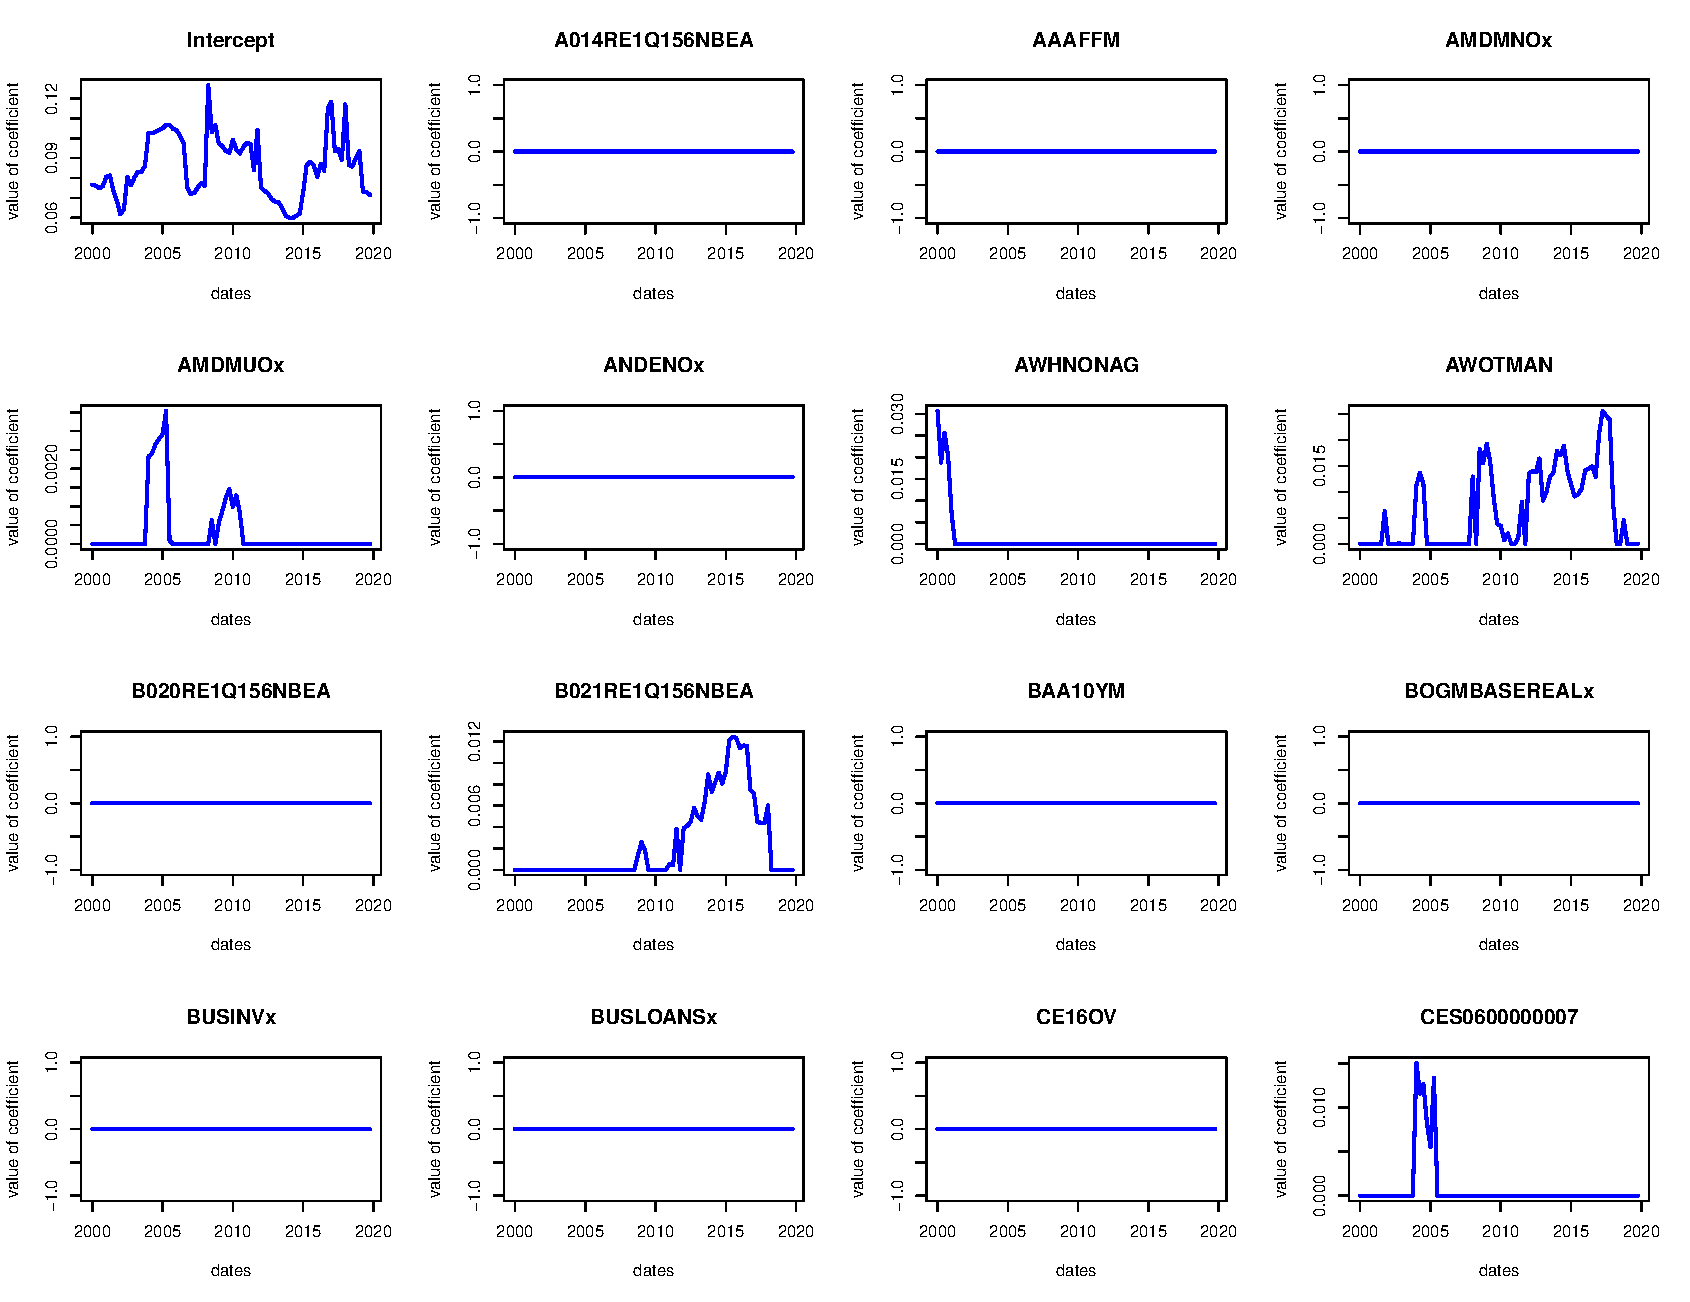
\includegraphics[page = 1, width=\textwidth]{plots/lasso_betas}
\caption{\label{first}Lasso regression: The evolution of the estimated $\beta$ coefficients over time}
\label{fig:lasso_betas}
\centering
\end{figure}

\begin{figure}[hbt!]
\includegraphics[page = 2, width=\textwidth]{plots/lasso_betas}
\caption{\label{second}Lasso regression: The evolution of the estimated $\beta$ coefficients over time}
\label{fig:lasso_betas}
\centering
\end{figure}

\begin{figure}[hbt!]
\includegraphics[page = 3, width=\textwidth]{plots/lasso_betas}
\caption{\label{third}Lasso regression: The evolution of the estimated $\beta$ coefficients over time}
\label{fig:lasso_betas}
\centering
\end{figure}

\begin{figure}[hbt!]
\includegraphics[page = 4, width=\textwidth]{plots/lasso_betas}
\caption{\label{fourth}Lasso regression: The evolution of the estimated $\beta$ coefficients over time}
\label{fig:lasso_betas}
\centering
\end{figure}

\begin{figure}[hbt!]
\includegraphics[page = 5, width=\textwidth]{plots/lasso_betas}
\caption{\label{fifth}Lasso regression: The evolution of the estimated $\beta$ coefficients over time}
\label{fig:lasso_betas}
\centering
\end{figure}

\begin{figure}[hbt!]
\includegraphics[page = 6, width=\textwidth]{plots/lasso_betas}
\caption{\label{sixth}Lasso regression: The evolution of the estimated $\beta$ coefficients over time}
\label{fig:lasso_betas}
\centering
\end{figure}

\begin{figure}[hbt!]
\includegraphics[page = 7, width=\textwidth]{plots/lasso_betas}
\label{fig:lasso_betas}
\caption{\label{seventh}Lasso regression: The evolution of the estimated $\beta$ coefficients over time}
\centering
\end{figure}

\begin{figure}[hbt!]
\includegraphics[page = 8, width=\textwidth]{plots/lasso_betas}
\caption{\label{eighth}Lasso regression: The evolution of the estimated $\beta$ coefficients over time}
\label{fig:lasso_betas}
\centering
\end{figure}

\begin{figure}[hbt!]
\includegraphics[page = 9, width=\textwidth]{plots/lasso_betas}
\label{fig:lasso_betas}
\caption{\label{ninth}Lasso regression: The evolution of the estimated $\beta$ coefficients over time}
\centering
\end{figure}

\begin{figure}[hbt!]
\includegraphics[page = 10, width=\textwidth]{plots/lasso_betas}
\caption{\label{tenth}Lasso regression: The evolution of the estimated $\beta$ coefficients over time}
\label{fig:lasso_betas}
\centering
\end{figure}

\begin{figure}[hbt!]
\includegraphics[page = 11, width=\textwidth]{plots/lasso_betas}
\label{fig:lasso_betas}
\caption{\label{eleventh}Lasso regression: The evolution of the estimated $\beta$ coefficients over time}
\centering
\end{figure}

\begin{figure}[hbt!]
\includegraphics[page = 12, width=\textwidth]{plots/lasso_betas}
\caption{\label{twelfth}Lasso regression: The evolution of the estimated $\beta$ coefficients over time}
\label{fig:lasso_betas}
\centering
\end{figure}

\begin{figure}[hbt!]
\includegraphics[page = 13, width=\textwidth]{plots/lasso_betas}
\label{fig:lasso_betas}
\caption{\label{thirteenth}Lasso regression: The evolution of the estimated $\beta$ coefficients over time}
\centering
\end{figure}

\end{subfigures}

\clearpage
%%%%%%%%%%%%%%%%%%%%%%
\begin{subfigures}
\begin{figure}[hbt!]
\includegraphics[page = 1, width=\textwidth]{plots/pca_loads}
\caption{\label{first}PCA: The evolution of the loading factors over time}
\label{fig:pca_loads}
\centering
\end{figure}

\begin{figure}[hbt!]
\includegraphics[page = 2, width=\textwidth]{plots/pca_loads}
\caption{\label{second}PCA: The evolution of the loading factors over time}
\label{fig:pca_loads}
\centering
\end{figure}

\begin{figure}[hbt!]
\includegraphics[page = 3, width=\textwidth]{plots/pca_loads}
\caption{\label{third}PCA: The evolution of the loading factors over time}
\label{fig:pca_loads}
\centering
\end{figure}

\begin{figure}[hbt!]
\includegraphics[page = 4, width=\textwidth]{plots/pca_loads}
\label{fig:pca_loads}
\caption{\label{fourth}PCA: The evolution of the loading factors over time}
\centering
\end{figure}

\begin{figure}[hbt!]
\includegraphics[page = 5, width=\textwidth]{plots/pca_loads}
\caption{\label{fifth}PCA: The evolution of the loading factors over time}
\label{fig:pca_loads}
\centering
\end{figure}

\begin{figure}[hbt!]
\includegraphics[page = 6, width=\textwidth]{plots/pca_loads}
\caption{\label{sixth}PCA: The evolution of the loading factors over time}
\label{fig:pca_loads}
\centering
\end{figure}

\begin{figure}[hbt!]
\includegraphics[page = 7, width=\textwidth]{plots/pca_loads}
\label{fig:pca_loads}
\caption{\label{seventh}PCA: The evolution of the loading factors over time}
\centering
\end{figure}

\begin{figure}[hbt!]
\includegraphics[page = 8, width=\textwidth]{plots/pca_loads}
\caption{\label{eighth}PCA: The evolution of the loading factors over time}
\label{fig:pca_loads}
\centering
\end{figure}

\begin{figure}[hbt!]
\includegraphics[page = 9, width=\textwidth]{plots/pca_loads}
\label{fig:pca_loads}
\caption{\label{ninth}PCA: The evolution of the loading factors over time}
\centering
\end{figure}

\begin{figure}[hbt!]
\includegraphics[page = 10, width=\textwidth]{plots/pca_loads}
\caption{\label{tenth}PCA: The evolution of the loading factors over time}
\label{fig:pca_loads}
\centering
\end{figure}

\begin{figure}[hbt!]
\includegraphics[page = 11, width=\textwidth]{plots/pca_loads}
\caption{\label{eleventh}PCA: The evolution of the loading factors over time}
\label{fig:pca_loads}
\centering
\end{figure}

\begin{figure}[hbt!]
\includegraphics[page = 12, width=\textwidth]{plots/pca_loads}
\caption{\label{twelfth}PCA: The evolution of the loading factors over time}
\label{fig:pca_loads}
\centering
\end{figure}

\begin{figure}[hbt!]
\includegraphics[page = 13, width=\textwidth]{plots/pca_loads}
\caption{\label{thirteenth}PCA: The evolution of the loading factors over time}
\label{fig:pca_loads}
\centering
\end{figure}

\end{subfigures}

\clearpage

\clearpage
%%%%%%%%%%%%%%%%%%%%%%
\begin{subfigures}
\begin{figure}[hbt!]
\includegraphics[page = 1, width=\textwidth]{plots/pls_loads}
\caption{\label{first}PLS: The evolution of the loading factors over time}
\label{fig:pls_loads}
\centering
\end{figure}

\begin{figure}[hbt!]
\includegraphics[page = 2, width=\textwidth]{plots/pls_loads}
\caption{\label{second}PLS: The evolution of the loading factors over time}
\label{fig:pls_loads}
\centering
\end{figure}

\begin{figure}[hbt!]
\includegraphics[page = 3, width=\textwidth]{plots/pls_loads}
\caption{\label{third}PLS: The evolution of the loading factors over time}
\label{fig:pls_loads}
\centering
\end{figure}

\begin{figure}[hbt!]
\includegraphics[page = 4, width=\textwidth]{plots/pls_loads}
\caption{\label{fourth}PLS: The evolution of the loading factors over time}
\label{fig:pls_loads}
\centering
\end{figure}

\begin{figure}[hbt!]
\includegraphics[page = 5, width=\textwidth]{plots/pls_loads}
\caption{\label{fifth}PLS: The evolution of the loading factors over time}
\label{fig:pls_loads}
\centering
\end{figure}

\begin{figure}[hbt!]
\includegraphics[page = 6, width=\textwidth]{plots/pls_loads}
\caption{\label{sixth}PLS: The evolution of the loading factors over time}
\label{fig:pls_loads}
\centering
\end{figure}

\begin{figure}[hbt!]
\includegraphics[page = 7, width=\textwidth]{plots/pls_loads}
\caption{\label{seventh}PLS: The evolution of the loading factors over time}
\label{fig:pls_loads}
\centering
\end{figure}

\begin{figure}[hbt!]
\includegraphics[page = 8, width=\textwidth]{plots/pls_loads}
\caption{\label{eighth}PLS: The evolution of the loading factors over time}
\label{fig:pls_loads}
\centering
\end{figure}

\begin{figure}[hbt!]
\includegraphics[page = 9, width=\textwidth]{plots/pls_loads}
\caption{\label{ninth}PLS: The evolution of the loading factors over time}
\label{fig:pls_loads}
\centering
\end{figure}

\begin{figure}[hbt!]
\includegraphics[page = 10, width=\textwidth]{plots/pls_loads}
\caption{\label{tenth}PLS: The evolution of the loading factors over time}
\label{fig:pls_loads}
\centering
\end{figure}

\begin{figure}[hbt!]
\includegraphics[page = 11, width=\textwidth]{plots/pls_loads}
\caption{\label{eleventh}PLS: The evolution of the loading factors over time}
\label{fig:pls_loads}
\centering
\end{figure}

\begin{figure}[hbt!]
\includegraphics[page = 12, width=\textwidth]{plots/pls_loads}
\caption{\label{twelfth}PLS: The evolution of the loading factors over time}
\label{fig:pls_loads}
\centering
\end{figure}

\begin{figure}[hbt!]
\includegraphics[page = 13, width=\textwidth]{plots/pls_loads}
\caption{\label{thirteenth}PLS: The evolution of the loading factors over time}
\label{fig:pls_loads}
\centering
\end{figure}

\end{subfigures}

\end{document}
